\documentclass[mathserif,11pt]{beamer}
%%%%%%%%%%%%%%%%%%%%%%%%%%%%%%%%%%%%%%%%%%%%%%%%%%%%%%%%%%%%%%%%%%%%%%%%%%%%%%%%%%%%%%%%%%%%%%%%%%%%%%%%%%%%%%%%%%%
% Appearance
\mode<presentation>
{
	\usetheme{CambridgeUS}
	\usecolortheme{whale}
	\setbeamercovered{transparent}
}
% Redefine beamer colors
% Captions and titles
\setbeamertemplate{caption}{\raggedright\insertcaption} 
\setbeamercolor{frametitle}{fg=cyan!90!black}
\setbeamercolor{title}{bg=cyan!90!black}

\setbeamercolor{palette primary}{fg=white, bg=cyan!70!black}
\setbeamercolor{palette secondary}{fg=white, bg=cyan!50!black}
\setbeamercolor{palette tertiary}{fg=white, bg=cyan!90!black}
% Outline slide
\setbeamertemplate{section in toc}[circle]
\setbeamerfont{section number projected}{family=\rmfamily,series=\bfseries,size=\normalsize}
\setbeamercolor{section number projected}{bg=cyan!90!black,fg=white}
% Itemize list
\setbeamertemplate{itemize item}[circle]
\setbeamertemplate{itemize subitem}[circle]
\setbeamercolor{itemize item}{fg=cyan!70!black}
\setbeamercolor{itemize subitemitem}{fg=cyan!90!black}
% Title box
\setbeamertemplate{frametitle}{%
	\nointerlineskip%
	\begin{beamercolorbox}[wd=\paperwidth,ht=2.0ex,dp=0.6ex]{frametitle}
		\hspace*{1ex}\insertframetitle%
	\end{beamercolorbox}%
}
%%%%%%%%%%%%%%%%%%%%%%%%%%%%%%%%%%%%%%%%%%%%%%%%%%%%%%%%%%%%%%%%%%%%%%%%%%%%%%%%%%%%%%%%%%%%%%%%%%%%%%%%%%%%%%%%%%%
\usepackage[english]{babel}
% or whatever
\usepackage[latin1]{inputenc}
% or whatever
\usepackage{array} % To vertically center tabular content 
\usepackage{times}
\usepackage[T1]{fontenc}
%\usepackage{eulervm}
%\usepackage{cmbright}
%%%%%%%%%%%%%%%%%%%%%%%%%%%%%%%%%%%%%%%%%%%%%%%%%%%%%%%%%%%%%%%%%%%%%%%%%%%%%%%%%%%%%%%%%%%%%%%%%%%%%%%%%%%%%%%%%%%%
%\usepackage{tikz}
\usepackage{pgfplots}
\pgfplotsset{every axis/.append style={line width=1pt}}
\usetikzlibrary{shapes,shadows,arrows,backgrounds,patterns,positioning,automata,calc,decorations.markings,decorations.pathreplacing,bayesnet,arrows.meta}
\usepackage{amsmath,amssymb,mathrsfs,amsfonts,amsthm} % for maths
\usepackage{graphicx}
%\usepackage{subfig}
\usepackage{eucal}    % for curly math letter symbols
\usepackage{amssymb}  % for ams symbols
\usepackage{pifont}
\usepackage{color} %Invoke options usenames,dvipsnames for larger color choice
\usepackage{microtype} % Slightly tweak font spacing for aesthetics
\usepackage{multicol} % Used for the two-column layout of the document
\usepackage{smartdiagram}
%%%%%%%%%%%%%%%%%%%%%%%%%%%%%%%%%%%%%%%%%%%%%%%%%%%%%%%%%%%%%%%%%%%%%%%%%%%%%%%%%%%%%%%%%%%%%%%%%%%%%%%%%%%%%%%%%%%%
\DeclareSymbolFontAlphabet{\mathcal} {symbols}
\DeclareSymbolFont{symbols}{OMS}{cm}{m}{n}
\DeclareMathAlphabet{\mathbfit}{OML}{cmm}{b}{it}
\newcommand\id{\ensuremath{\mathbbm{1}}} 
\DeclareMathOperator{\E}{\mathbb{E}}
\DeclareMathOperator{\eye}{\mathbb{I}}
\DeclareMathOperator{\zeros}{\mathbb{O}}
\DeclareMathOperator{\tr}{\textrm{tr}}
\DeclareMathOperator{\vvec}{\textrm{vec}}
\DeclareMathOperator{\ik}{\mathrm{k}}
\DeclareMathOperator{\ip}{\mathrm{p}}
\DeclareMathOperator{\inn}{\mathrm{n}}
\DeclareMathOperator{\im}{\mathrm{m}}
\DeclareMathOperator{\td}{\mathrm{t}}
\DeclareMathOperator{\kd}{\mathrm{k}}
\DeclareMathOperator{\T}{\mathrm{T}}
\DeclareMathOperator{\K}{\mathrm{K}}
%%%%%%%%%%%%%%%%%%%%%%%%%%%%%%%%%%%%%%%%%%%%%%%%%%%%%%%%%%%%%%%%%%%%%%%%%%%%%%%%%%%%%%%%%%%%%%%%%%%%%%%%%%%%%%%%%%%%
\usepackage[backend=bibtex,style=ieee]{biblatex} % bibliography
\bibliography{Bibliography-thesis}
\renewcommand*{\bibfont}{\footnotesize}
%%%%%%%%%%%%%%%%%%%%%%%%%%%%%%%%%%%%%%%%%%%%%%%%%%%%%%%%%%%%%%%%%%%%%%%%%%%%%%%%%%%%%%%%%%%%%%%%%%%%%%%%%%%%%%%%%%%%
\title[Identification of immune cell migration] % (optional, use only with long paper titles)
{Modelling and Identification of Immune Cell Migration during the Inflammatory Response}
\subtitle{PhD Viva (extended version)}
\author[A. Kadochnikova]{A. Kadochnikova\inst{1}}
\institute[ACSE,TUoS]{\inst{1}
  Department of Automatic Control and Systems Engineering\\
  The University of Sheffield}
\date[21/06/2019]{21 June 2019}

\pgfdeclareimage[height=1cm]{university-logo}{UoSarms.pdf}
\logo{\pgfuseimage{university-logo}}

\begin{document}
\begin{frame}
  \titlepage
\end{frame}
\begin{frame}{Outline}
  \tableofcontents[hideallsubsections]
  % You might wish to add the option [pausesections]
\end{frame}

% - Exactly two or three sections (other than the summary).
% - At *most* three subsections per section.
% - Talk about 30s to 2min per frame. So there should be between about
%   15 and 30 frames, all told.


%% Chapters 1-2
\section[Background]{Background \& Motivation}
\subsection{Neutrophils in inflammation}
\begin{frame}
\begin{itemize}
	\item The process of inflammation is driven by rapid migration of neutrophils towards and away from the infectious area.
	\item Chemotaxis - directed migration in response to chemical attractants - is the dominant mechanism of neutrophil recruitment.
	\item Neutrophil reverse migration hypotheses: driven away by repellents vs. random redistribution.
	\item Cell locomotion is linked to gradient sensing by changes in subcellular concentrations of various messengers.
	\item Majority of therapeutic treatments of inflammation rely on manipulating cells' presentation of their environment. 
\end{itemize}
Mathematical modelling is a standard method for characterisation of the experimental data.
\end{frame}
\subsection{Identified gaps in literature}
\begin{frame}
General problem: abundance of mathematical models without predictive capability.\\
\vspace{0.2cm}
Specific gaps in literature:
\begin{itemize}
	\item Chemoattractant concentrations must be inferred from \textit{in vivo} experiments.
	\item Random walk models do not provide insight into global environment influence.
	\item No studies contemplating the possibility heterogeneous cell behaviour during the resolution stage.
	\item PIP$_3$ is often assumed as the primary subcellular regulator without experimental evidence.
\end{itemize}
\vspace{0.2cm}
\centering
\only<1>{\large{Common concept:\\ Complicated model $\rightarrow$ Realistic simulations.}}\only<2>{\large{Systematic approach:\\ Simplified models $\rightarrow$ Linking to data $\rightarrow$ Meaningful perditions.}}
\end{frame}
\subsection{Research Objectives}
\begin{frame}
Objectives:
\begin{itemize}
	\item Develop a dynamical model that describes cell interaction with the acting environment.
	\item Data-driven estimation of global chemoattractant concentration field and cell behavioural modes.
	\item Parameter estimation of neutrophil morphodynamics model.
\end{itemize}
\vspace{0.3cm}
Restrictions:
  \begin{itemize}
  	\item Minimise prior assumptions about the shape of the environment.
  	\item Minimise prior assumptions about the subcellular regulators.
  	\item Ensure identifiability of models by keeping the number of unknown parameters low. 
  	\end{itemize}
\end{frame}
%% Chapters 3-5
\section{Environment inference: homogeneous cell behaviour}
\subsection{Problem statement}
\begin{frame}
\begin{columns}
	\begin{column}{0.55\textwidth}
		\centering
		\only<1>{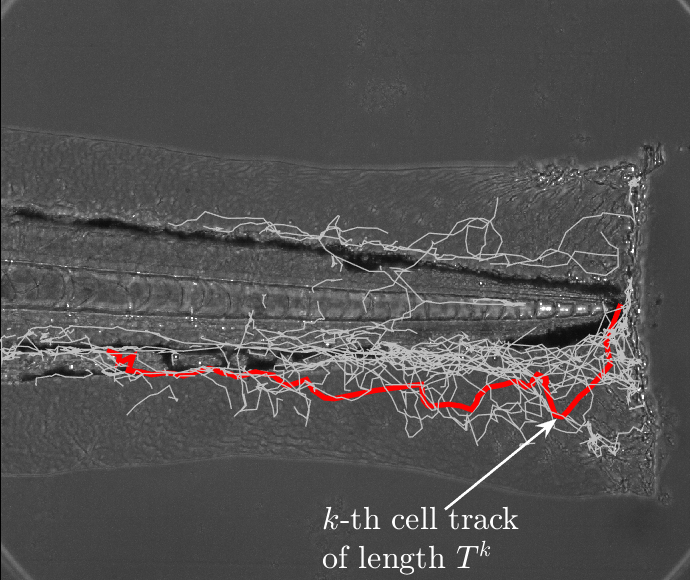
\includegraphics[scale=0.35]{Figures/track_k.png}}\only<2-4>{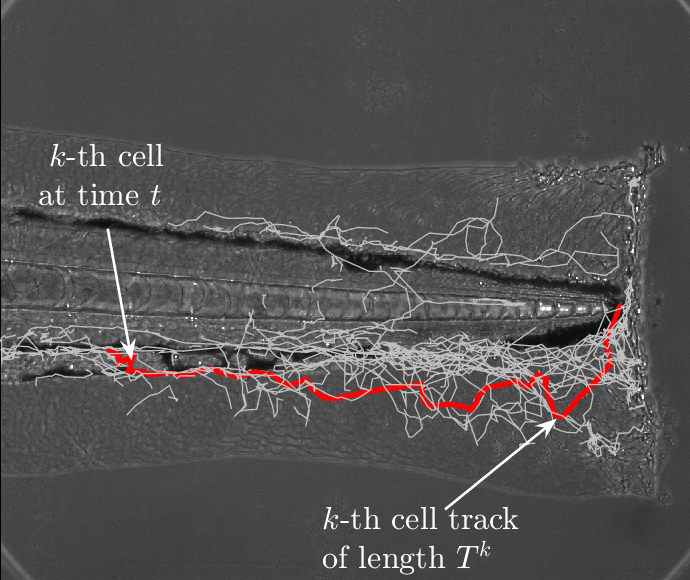
\includegraphics[scale=0.35]{Figures/track_k_time_t.png}}\only<5->{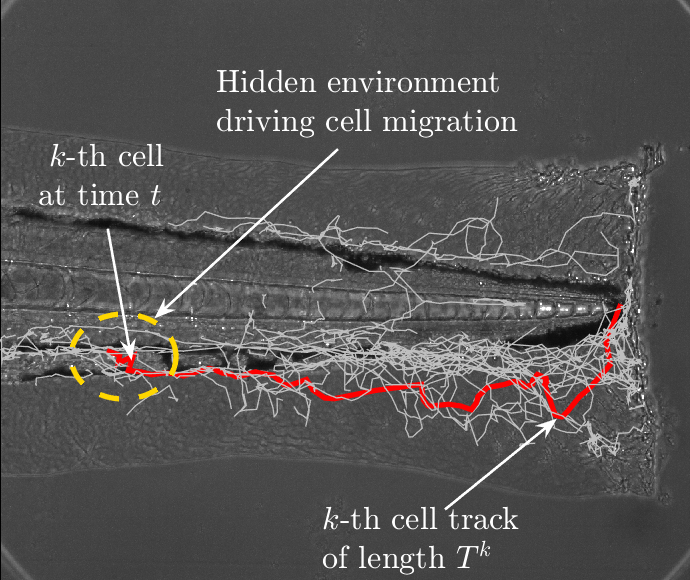
\includegraphics[scale=0.35]{Figures/track_filed.png}}
	\end{column}
	\begin{column}{0.42\textwidth}
		Time series data:
		\begin{itemize}
			\item<1-> $K$ tracks: $\mathcal{Y} = \{\mathbf{y}^{k} \}^{K}_{k=1}$
			\item<2-> Single track: $\mathbf{y}^{k} = \{ \mathbfit{y}^{k}_{t}\}^{T^k}_{t=1}$
			\item<3-> Single data point: $\mathbfit{y}^{k}_{t} = \left[ \bar{s}_{\mathrm{x}}, \bar{s}_{\mathrm{y}} \right]^{\top}$
			\item<4-> Full state: $\mathbfit{x}^{k}_{t} = \left[ s_{\mathrm{x}}, s_{\mathrm{y}}, v_{\mathrm{x}}, v_{\mathrm{y}} \right]^{\top}$
			\item<5-> Environment influence:
			$\mathbfit{u}^{k}_{t} = \mathbfit{u}^{k}_{t}(\mathbfit{s}) = \nabla \mathcal{U}(\mathbfit{s}).$
		\end{itemize}
	\end{column}
\end{columns}
\bigskip
\uncover<6->{1. Develop a parametrised finite-order model of global $\mathcal{U}(\mathbfit{s})$.\\}
\bigskip
\uncover<7->{2. Estimate hidden global $\mathcal{U}(\mathbfit{s})$ from localised data $\mathcal{Y}$.}
\end{frame}
\begin{frame}{Defining assumptions}
\begin{itemize}
	\item A migrating call is moving as a massive Brownian particle:
	\begin{equation*}
	\dot{v}(t)= - \rho v(t) + \sqrt{\sigma}\mathbf{W}(t).
	\end{equation*}
	\item Each cell at each time is moving in response to the acting environment:
	\begin{equation*}
	\dot{v}(t) = - \rho v(t) + \sqrt{\sigma}\mathbf{W}(t) + {\psi}(t).
	\end{equation*}
	\item Hidden chemoattractant environment is acting on cells as a potential field:
	\begin{equation*}
	\dot{v}(t) = - \rho v(t) + \sqrt{\sigma}\mathbf{W}(t) + \nabla\mathcal{U}(s(t)).
	\end{equation*}
	\item Hidden chemoattractant environment is time-invariant:
	\begin{equation*}
	\mathcal{U}(t) = const.
	\end{equation*}
\end{itemize}
\end{frame}
\subsection{Methods}
\begin{frame}{Decomposition of the environment}
\begin{columns}
\begin{column}{0.4\textwidth}
	\centering
	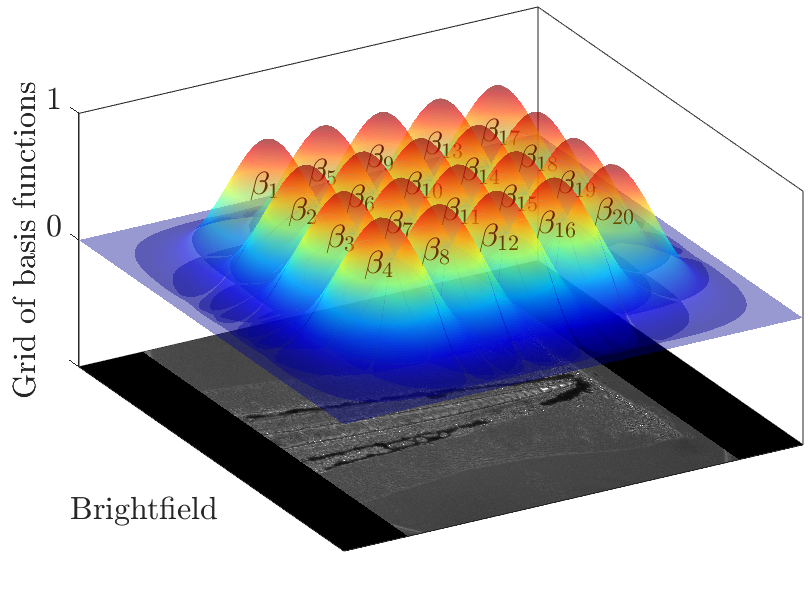
\includegraphics[scale=0.2]{Figures/grid.png}\\
	\footnotesize{a) 5x4 grid of tensor B-splines}
	\hfil
	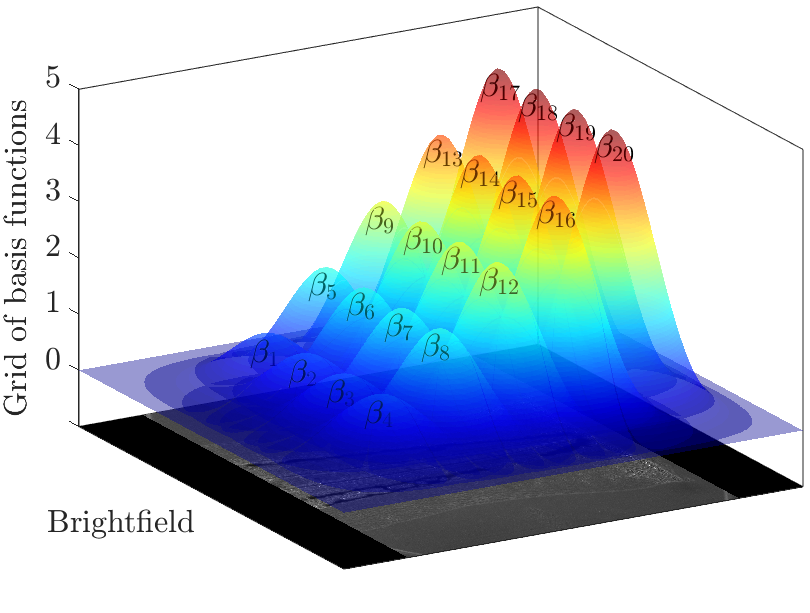
\includegraphics[scale=0.2]{Figures/grid2.png}\\
	\footnotesize{b) $\theta_h$ defines magnitude of $\beta_h (s_{\mathrm{x}}, s_{\mathrm{y}})$}
\end{column}
\begin{column}{0.5\textwidth}
	\centering
	\vspace{-0.5cm}
	\begin{equation*}\label{eq_field}
	\mathcal{U}(s_{\mathrm{x}}, s_{\mathrm{y}}) = \mathcal{B}\Theta = \sum_{h=1}^{N_b}\beta_h(s_{\mathrm{x}}, s_{\mathrm{y}})\theta_h,
	\end{equation*}
	\vspace{-0.5cm}
	\begin{subequations}
		\begin{eqnarray*}
		\Theta &= \left[\theta_1,\dots,\theta_h,\dots,\theta_{N_b}\right]^{\top},\\
		\mathcal{B} &= \left[\beta_1,\dots,\beta_h,\dots,\beta_{N_b}\right],\\
		\beta_h &(s_{\mathrm{x}}, s_{\mathrm{y}}) = \beta^{4}_{l}(s_{\mathrm{x}})\beta^{4}_{m}(s_{\mathrm{y}}).
		\end{eqnarray*}
	\end{subequations}

	\vfil
	\vspace{0.3cm}
	\only<1>{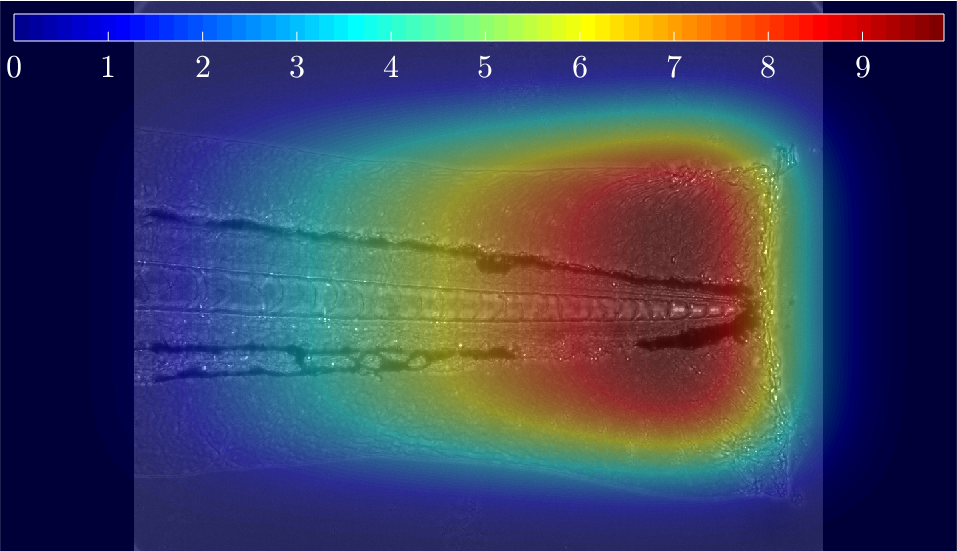
\includegraphics[scale=0.2]{Figures/grid2_heatmap.png}}
	\only<2>{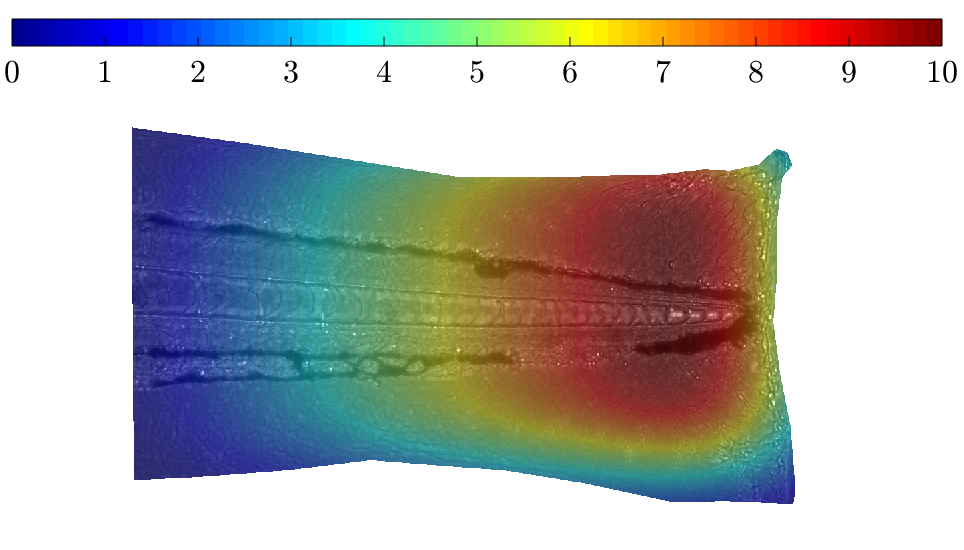
\includegraphics[scale=0.2]{Figures/grid_mask.png}}\\
	\footnotesize{Example of the resultant field.}
\end{column}	
\end{columns}
\end{frame}
\begin{frame}{Model of neutrophil dynamics}
\vspace{-0.1cm}
Discrete time SSM of the $\kd$-th cell :
\begin{equation*}\label{eq_dyn}
\mathbfit{x}^{\kd}_{\td} = A \mathbfit{x}^{\kd}_{\td-1} + B\phi_{\td-1}^{\kd}(s_{\mathrm{x}},s_{\mathrm{y}}) \Theta + G\mathbfit{w}^{\kd}_{\td-1}, \quad \mathbfit{w}^{\kd}_{\td} \sim \mathcal{N}(0, Q)
\end{equation*}
\begin{equation*}\label{eq_meas}
\mathbfit{y}^{\kd}_{\td} = C\mathbfit{x}^{\kd}_{\td} + \mathbfit{v}^{\kd}_{\td}, \quad \mathbfit{v}^{\kd}_{\td} \sim \mathcal{N}(0, R)
\end{equation*}
where
\begin{equation*}
\phi_{\td}^{\kd}(s_{\mathrm{x}},s_{\mathrm{y}}) = \nabla \mathcal{B}(s_{\mathrm{x}}, s_{\mathrm{y}}) = \left[\begin{array}{ccccc} \frac{ \partial\beta_1(s_{\mathrm{x}},s_{\mathrm{y}}) }{\partial s_{\mathrm{x}}} &
 \dots &\frac{ \partial\beta_h(s_{\mathrm{x}},s_{\mathrm{y}}) }{\partial s_{\mathrm{x}}}& \dots&\frac{ \partial\beta_{N_b}(s_{\mathrm{x}},s_{\mathrm{y}}) }{\partial s_{\mathrm{x}}} \\
\frac{ \partial\beta_1(s_{\mathrm{x}},s_{\mathrm{y}}) }{\partial s_{\mathrm{y}}} & \dots &\frac{ \partial\beta_h(s_{\mathrm{x}},s_{\mathrm{y}}) }{\partial s_{\mathrm{y}}}& \dots&\frac{ \partial\beta_{N_b}(s_{\mathrm{x}},s_{\mathrm{y}}) }{\partial s_{\mathrm{y}}}
\end{array}\right]. 
\end{equation*}
\begin{equation*}
A = \left[\begin{array}{cc}
\eye & T\eye \\
\zeros & (1-T\rho) \eye
\end{array}\right]; 
\hfil 
B = \left[\begin{array}{c}
\zeros \\ T \eye
\end{array}\right];
\hfil
G = \left[ \begin{array}{c}
\zeros \\ T\eye
\end{array} \right]; 
\hfil
C = \left[ \begin{array}{cc}
\eye & \zeros
\end{array}\right].
\end{equation*}
\vspace{0.3cm}
SSM is linear in $\Theta$ and non-linear in $\mathbfit{x}$.   
\end{frame}
\begin{frame}{Approximate EM framework}
E-step:
\vspace{-0.5cm}
\begin{equation*}
\mathcal{Q}(\Theta, \hat{\Theta}^i) = \E \big[\log p(\Theta \mid \mathcal{Y}) \big] = \E \Big[ \sum_{\kd=1}^{\K} \sum_{\td=1}^{\T_{\kd}}\log p(\mathbfit{x}_{\td}^{\kd} \mid \mathbfit{x}_{\td-1}^{\kd}, \Theta) \mid \mathcal{Y}, \hat{\Theta}^{i} \Big] + c.
\end{equation*}
\vspace{-0.2cm}
\begin{equation*}
p(\mathbfit{x}_{\td}^{\kd} \mid \mathbfit{x}_{\td-1}^{\kd} \Theta) = \mathcal{N}\big((G)^\dag \left\lbrace  \mathbfit{x}_{\td}^{\kd}- A\mathbfit{x}_{\td-1}^{\kd}- B\phi(C\mathbfit{x}_{\td-1}^{\kd}) \Theta\right\rbrace , \Sigma_{\mathbfit{w}}\footnote{\scriptsize{$\Sigma_{\mathbfit{w}} \triangleq \big\{(G)^\dag \big\}^\top (Q_{\omega})^{-1} (G)^\dag$}}\big).
\end{equation*}
\vfil
Forecasting step:
\vspace{-0.2cm}
\begin{equation*}
\mathbfit{s}_{\td}^{\kd} = C \hat{\mathbfit{x}}_{\td \mid \T^{\kd}}^{\kd}, \quad \td = 1, \dots, \T^{\kd}, \kd = 1, \dots, \K.
\end{equation*} 
\vspace{-0.4cm}
\begin{equation*}
\begin{split}
p(\mathbfit{x}_{\td}^{\kd} \mid \mathbfit{x}_{\td-1}^{\kd}, \Theta) &\approx p(\mathbfit{x}_{\td}^{\kd} \mid \mathbfit{x}_{\td-1}^{\kd}, \mathbfit{s}_{\td-1}^{\kd}, \Theta)\\ &=   \mathcal{N}\big((G)^\dag\left\lbrace  \mathbfit{x}_{\td}^{\kd}- A\mathbfit{x}_{\td-1}^{\kd}- B\phi(\mathbfit{s}_{\td-1}^{\kd}) \Theta\right\rbrace, \Sigma_{\mathbfit{w}}\big).
\end{split}
\end{equation*}
M-step:\\
\vspace{-0.5cm}
\begin{equation*}
\hat{\Theta}^{i+1} = \arg \underset{\Theta}{\max} \tilde{\mathcal{Q}}(\Theta, \hat{\Theta}^i).
\end{equation*}
\end{frame}
\subsection{Selected results}
\begin{frame}{Inferred chemoattractant concentration}
\begin{columns}
	\begin{column}{0.3\textwidth}
		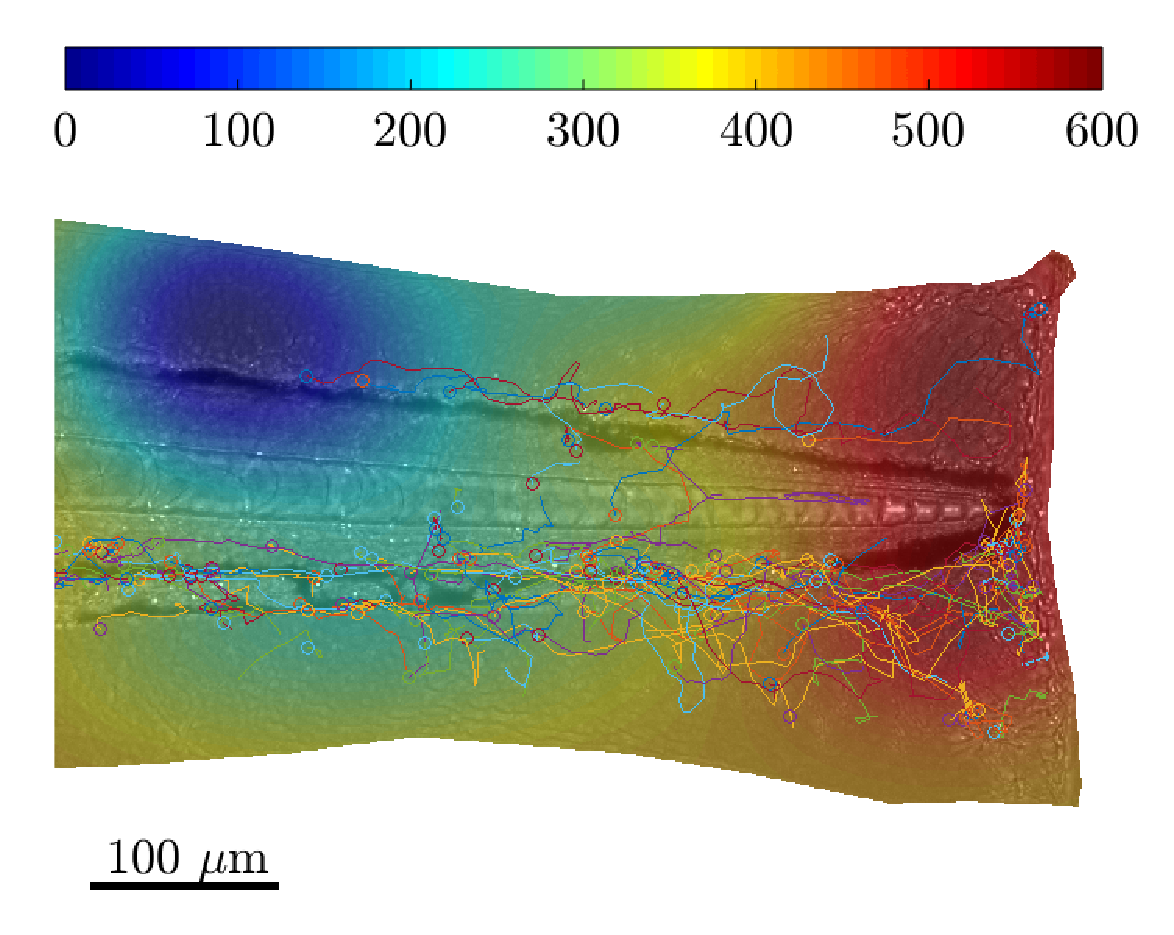
\includegraphics[scale=0.19]{Figures/field_tracks_1.png}
		\vspace{0.4cm}
		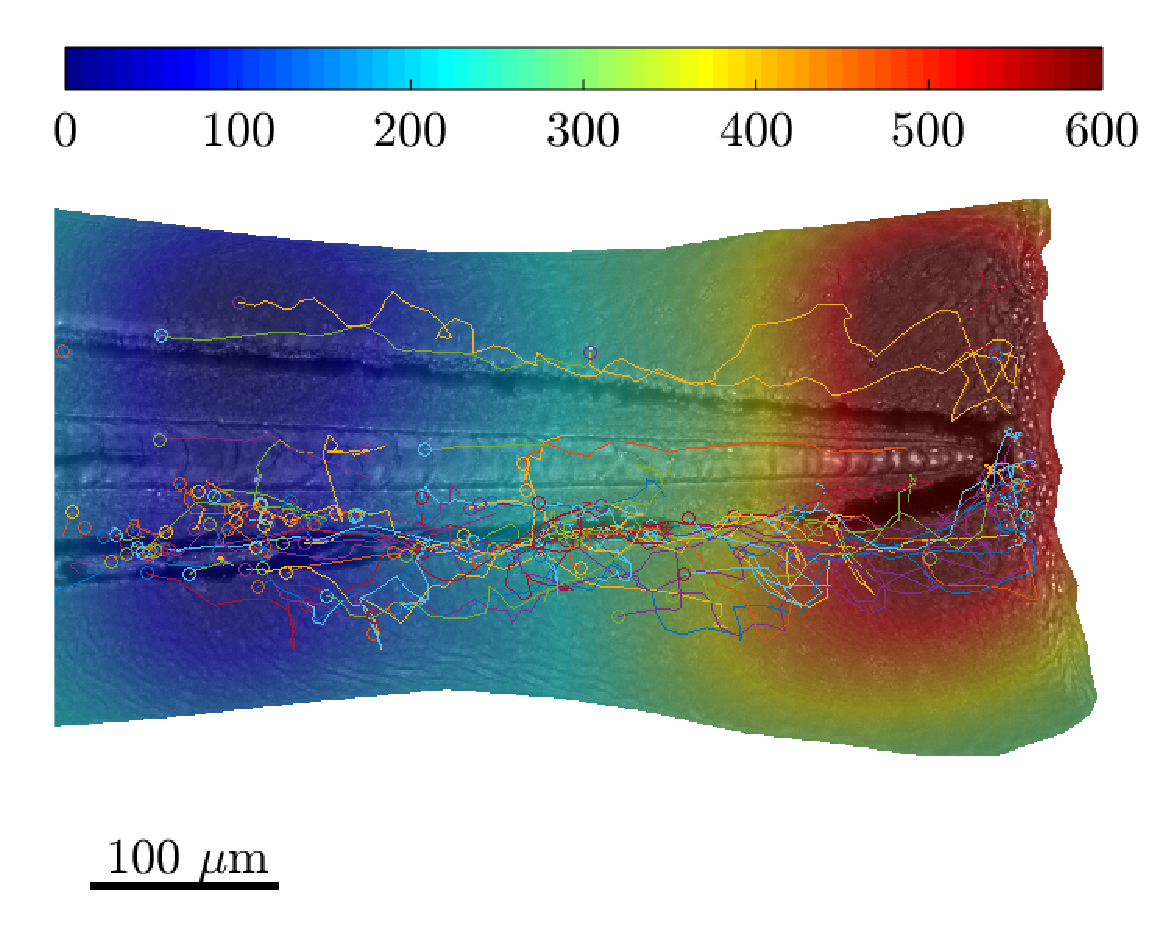
\includegraphics[scale=0.19]{Figures/field_tracks_3.png}
	\end{column}
	\begin{column}{0.3\textwidth}
		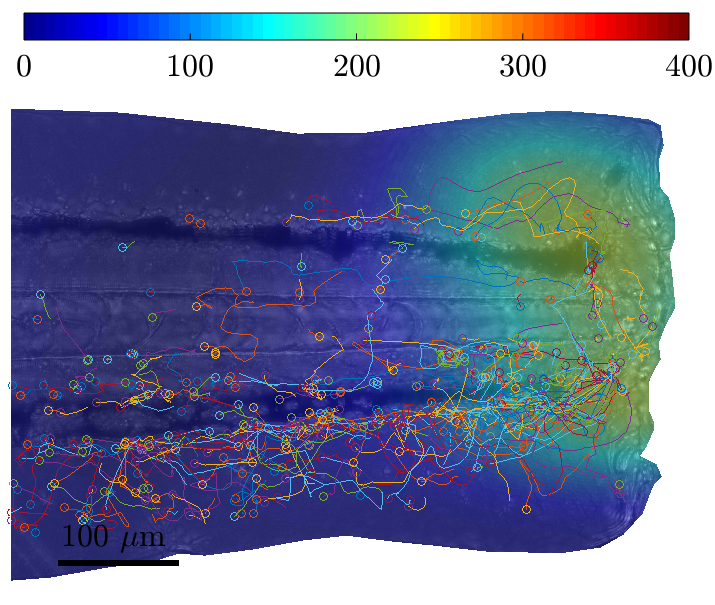
\includegraphics[scale=0.185]{Figures/s2_ukf_tracks.png}
		\vspace{0.3cm}
		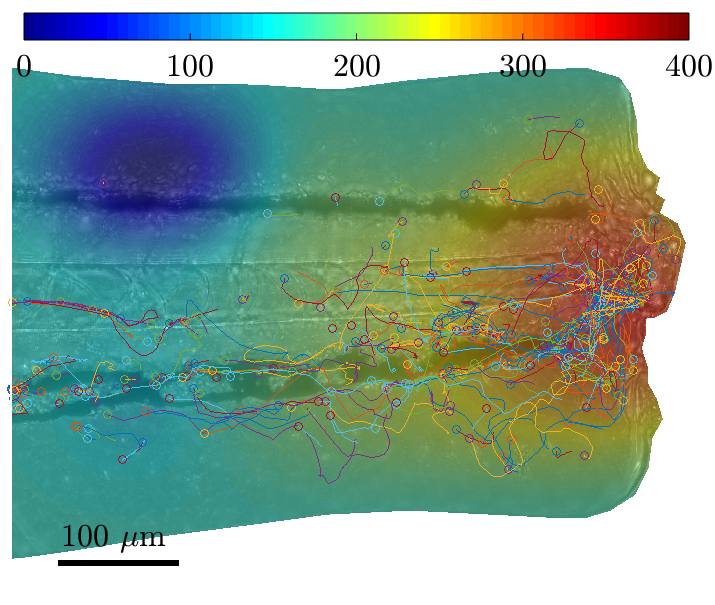
\includegraphics[scale=0.185]{Figures/s3_ukf_tracks.png}
	\end{column}
	\begin{column}{0.3\textwidth}
		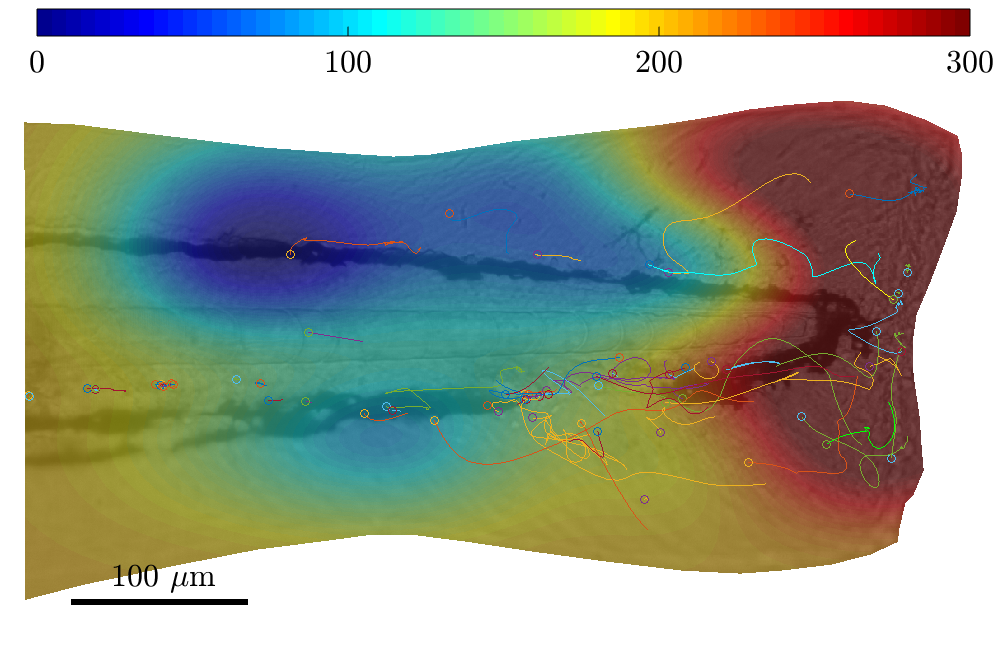
\includegraphics[scale=0.14]{Figures/n3_p1_ukf_tracks.png}
		\vspace{0.6cm}
		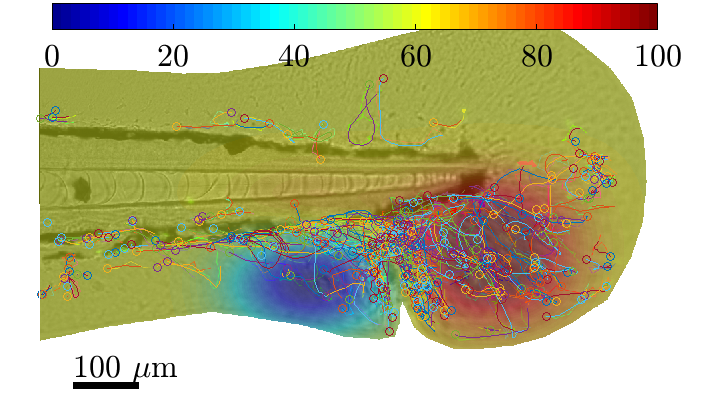
\includegraphics[scale=0.2]{Figures/nick4_4x4_05.png}
	\end{column}
\end{columns}
\begin{columns}
	\begin{column}{0.3\textwidth}
		\centering
		\footnotesize{ a) normal injury}\\
		\footnotesize{(6 datasets)}
	\end{column}
	\begin{column}{0.3\textwidth}
		\centering
	\footnotesize{ b) severe injury}\\
	\footnotesize{(2 datasets)}
\end{column}
	\begin{column}{0.3\textwidth}
		\centering
	\footnotesize{ c) mild injury}\\
	\footnotesize{(6 datasets)}
\end{column}
\end{columns}
\end{frame}
\begin{frame}{Estimated cell velocities}
\begin{columns}
	\begin{column}{0.33\textwidth}
		\scalebox{0.7}{\input{Tikzes/histogram_vx.tikz}}\vfil
		\scalebox{0.7}{\input{Tikzes/histogram_vy.tikz}}
	\end{column}
	\begin{column}{0.3\textwidth}
		\scalebox{0.7}{\input{Tikzes/histogram_vx_severe.tikz}}\vfil
		\scalebox{0.7}{\input{Tikzes/histogram_vy_severe.tikz}}
	\end{column}
	\begin{column}{0.3\textwidth}
		\scalebox{0.7}{\input{Tikzes/histogram_vx_nicked.tikz}}\vfil
		\scalebox{0.7}{\input{Tikzes/histogram_vy_nicked.tikz}}
	\end{column}
\end{columns}
\begin{columns}
	\centering
	\begin{column}{0.33\textwidth}
		\centering
		\footnotesize{ a) normal injury}
	\end{column}
	\begin{column}{0.3\textwidth}
		\centering
		\footnotesize{ b) severe injury}
	\end{column}
	\begin{column}{0.3\textwidth}
		\centering
		\footnotesize{ c) mild injury}
	\end{column}
\end{columns}
\end{frame}
%\begin{frame}{Cell modes}
%Neutrophil behaviour during recruitment stage can be described by a set of models.
%\begin{columns}
%	\begin{column}{0.5\textwidth}
%		Types of random walk \cite{Jones2015}:
%		\begin{itemize}
%			\item biased, persistent
%			\item biased, non-persistent
%			\item non-biased, persistent
%			\item non-biased, non-persistent
%		\end{itemize}
%	\end{column}
%	\begin{column}{0.5\textwidth}
%		Based on the interaction \\with the environment:
%		\begin{itemize}
%			\item driven by the field
%			\begin{itemize}
%				\item KS model
%				\item Potential Field model
%			\end{itemize}
%			\item insensitive - RW
%			\item stationary - RW
%		\end{itemize}
%		
%	\end{column}
%\end{columns}
%\end{frame}

\section{Environment inference: heterogeneous cell behaviour}
\subsection{Problem statement}
\begin{frame}
\begin{columns}
	\begin{column}{0.5\textwidth}
		\centering
		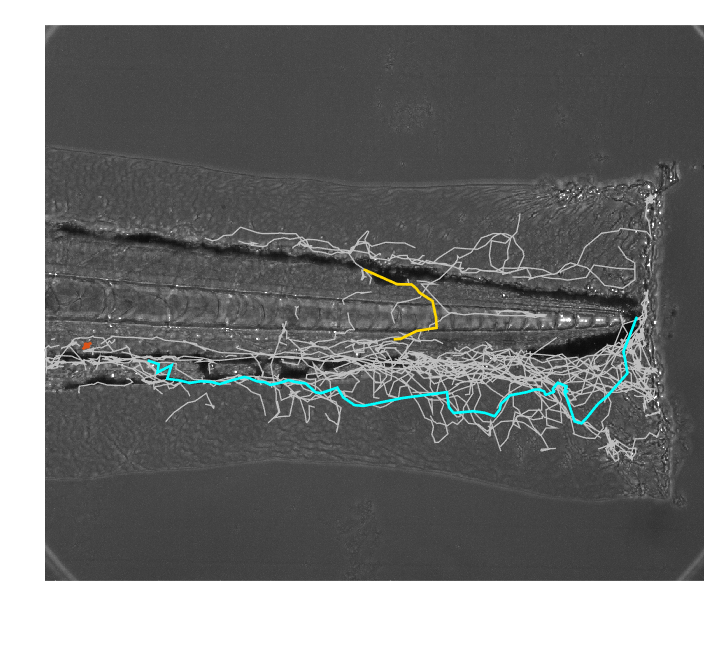
\includegraphics[scale=0.31]{Figures/example_tracks.png}
	\end{column}
	\begin{column}{0.5\textwidth}
		\centering
		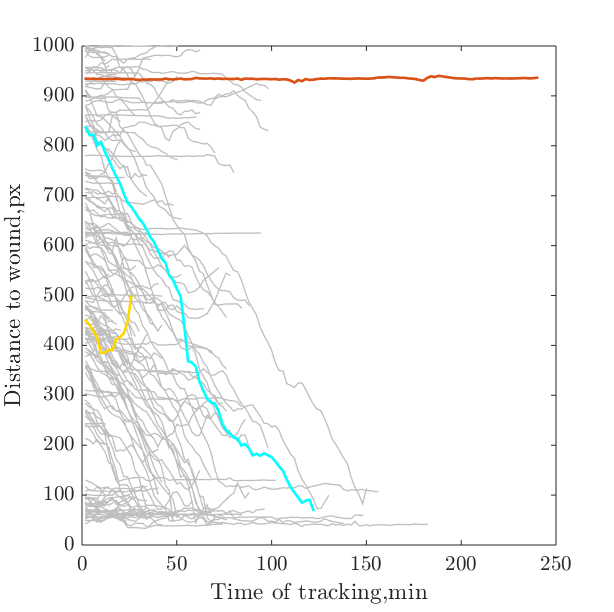
\includegraphics[scale=0.34]{Figures/example_distances.png}
		\vspace{0.29cm}
	\end{column}
\end{columns}
Neutrophil behaviour is not uniform.\\
\vspace{0.2cm}
\uncover<2->{1. Does a cell at a given time interact with the environment $\mathcal{U}(\mathbfit{s})$?\\}
\vspace{0.2cm}
\uncover<3->{2. Estimate hidden global $\mathcal{U}(\mathbfit{s})$ from the interaction with responsive  cells.}
\end{frame}
\begin{frame}{Defining assumptions (upd.)}
Remain the same:
\begin{itemize}
	\item Each migrating call is moving as a massive Brownian particle.
	\item Hidden chemoattractant environment is acting on migrating cells as a potential field.
	\item Hidden chemoattractant environment is time-invariant.
\end{itemize}
\vspace{0.3cm}
Relaxed assumptions:
\begin{itemize}
	\item Each migrating cell at any time can be in one of free modes: stationary, responsive or non-responsive.
	\item Switching between modes happens randomly.
	\item Each behavioural mode can be reached from any other mode.
\end{itemize}
\end{frame}
\subsection{Methods}
\begin{frame}{Jump Markov system}
\vspace{-1cm}
\begin{equation*}\label{eq_dyn1}
\mathbfit{x}_{\td}^{\kd} = A(M^j)\mathbfit{x}_{\td-1}^{\kd} + B(M^j)\phi_{\td-1}^{\kd}(s_{\mathrm{x}},s_{\mathrm{y}}) \Theta + G(M^j)\mathbfit{w}_{\td-1}^{\kd}, \quad \mathbfit{w}_{\td}^{\kd} \sim \mathcal{N}(0,Q(M^j)).
\end{equation*}
\begin{columns}
	\begin{column}{0.55\textwidth}
	\footnotesize{
	Cell modes:
	\begin{align*}
	M^1&: A = \left[\begin{array}{cc}
	\eye & T\eye \\
	\zeros & (1-T\rho(M^1)) \eye
	\end{array}\right] 
	\hfil 
	B = \left[\begin{array}{c}
	\zeros \\ T \eye
	\end{array}\right]
	\\
	M^2&: A = \left[\begin{array}{cc}
	\eye & T\eye \\
	\zeros & (1-T\rho(M^2)) \eye
	\end{array}\right]
	\hfil 
	B = \left[\begin{array}{c}
	\zeros \\ \zeros
	\end{array}\right]
	\\
	M^3&: A = \left[\begin{array}{cc}
	\eye & T\eye \\
	\zeros & (1-T\rho(M^3)) \eye
	\end{array}\right]
	\hfil 
	B = \left[\begin{array}{c}
	\zeros \\ \zeros
	\end{array}\right]
	\\
	Q&(M^3) \ll Q(M^1) < Q(M^2).
	\end{align*}
}
\end{column}
\begin{column}{0.45\textwidth}
	\scalebox{0.58}{\input{Tikzes/Markov_chain_switch.tikz}}
\end{column}
\end{columns}
\end{frame}

%\begin{frame}{Jump Markov Linear System}
%\begin{columns}
%\begin{column}{0.6\textwidth}
%\scalebox{0.8}{\input{Tikzes/Markov_chain_switch.tikz}}
%\end{column}
%\begin{column}{0.4\textwidth}
%\begin{itemize}
%	\item \textit{k} - cell index
%	\item t - time 
%	\item $\pi_j$ - probability of $M^j$ at time $t = 0$
%	\item $\phi_{ij}$ - probability of transitioning from $M^i$ to $M^j$
%	\item $\psi_j$ - probability of state $x^{k}_{t}$	
%\end{itemize}
%\end{column}
%\end{columns}
%\end{frame}
%
%
\begin{frame}{Inference framework}
\begin{figure}
\centering
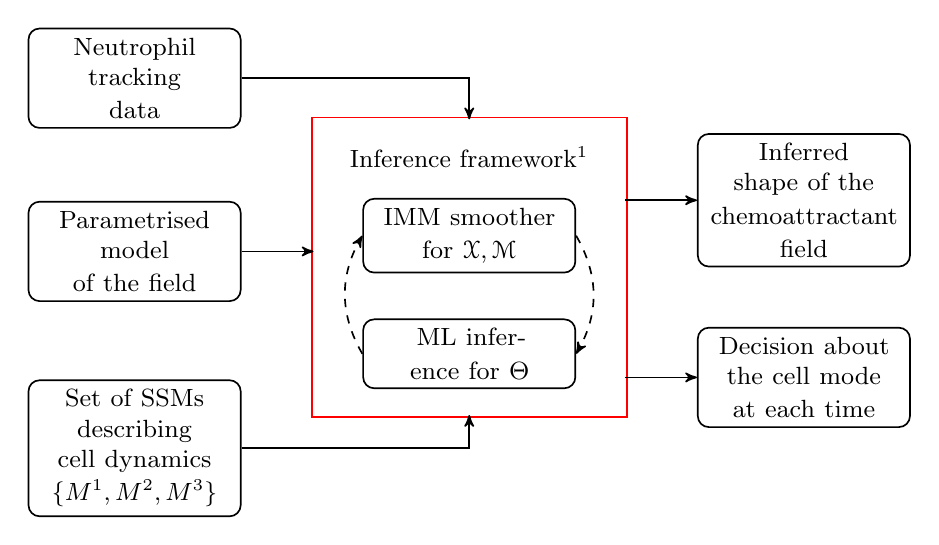
\begin{tikzpicture}[->, >=stealth', auto, semithick, node distance=5em]
\tikzstyle{block} = [rectangle, draw, fill=white, 
text width=7em, text centered, rounded corners, minimum height=2em]
\tikzstyle{line} = [draw, -latex']	
\node[block,align=center] at (1.5,7) (A1){\small Neutrophil tracking \\ data};
\node[block,align=center] at (1.5,4.8) (A2){\small Parametrised model \\ of the field};
\node[block,align=center] at (1.5,2.3) (A3){\small Set of SSMs describing\\ cell dynamics \\ $\{M^1, M^2, M^3\}$};
\node[align=center] at (5.75,6) (A4){\small Inference framework\footnote{\scriptsize{The framework is derived and validated on MC simulations in Chapter 4.}}};
\node[block,align=center] at (5.75,5) (A5){\small  IMM smoother for $\mathcal{X},\mathcal{M}$};
\node[block,align=center] at (5.75,3.5) (A6){\small ML inference for $\Theta$};
\node[block,align=center] at (10,5.45) (A7){\small Inferred shape of the\\chemoattractant field};
\node[block,align=center] at (10,3.2) (A8){\small Decision about\\ the cell mode\\ at each time};
\draw[red] (3.75,6.5) rectangle (7.75,2.7);
\node at (5.75,6.35) (A9){};
\node at (5.75,2.85) (A10){};
\node at (3.9,4.8) (A11){};
\node at (7.6,5.45) (A12){};
\node at (7.6,3.2) (A13){};
%% arrows
\draw (A1) -| (A9); 
\draw (A2) -- (A11); 
\draw (A3) -| (A10); 
\draw (A12) -- (A7); 
\draw (A13) -- (A8); 
\path
(A5.east) edge[dashed,bend left=30] (A6.east);
\path
(A6.west) edge[dashed,bend left=30] (A5.west);
\end{tikzpicture}
\end{figure}
\end{frame}

\subsection{Selected results}
\begin{frame}{Migratory modes - normal injury}
\begin{columns}
	\begin{column}{0.31\textwidth}
		\vspace{-0.2cm}
		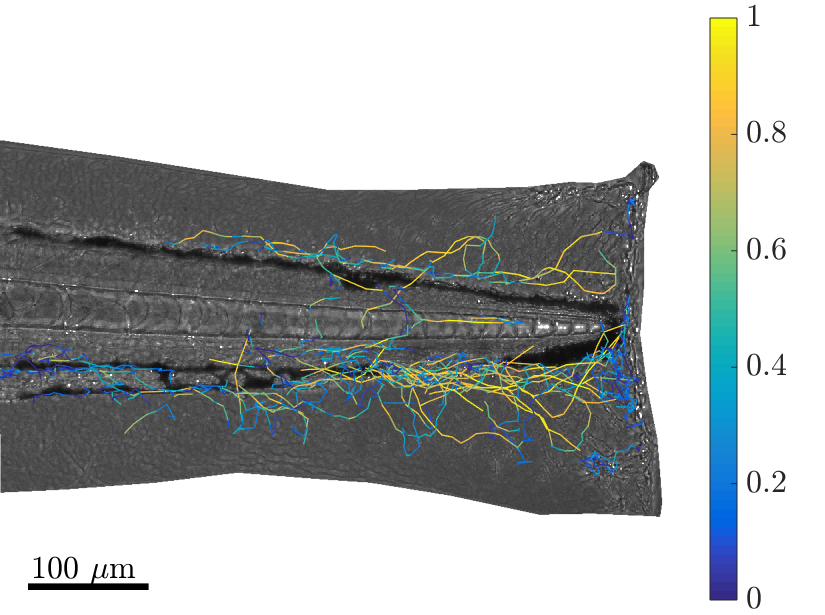
\includegraphics[scale=0.19]{Figures/mode1_fish1.png}\vfil
		\vspace{0.2cm}
		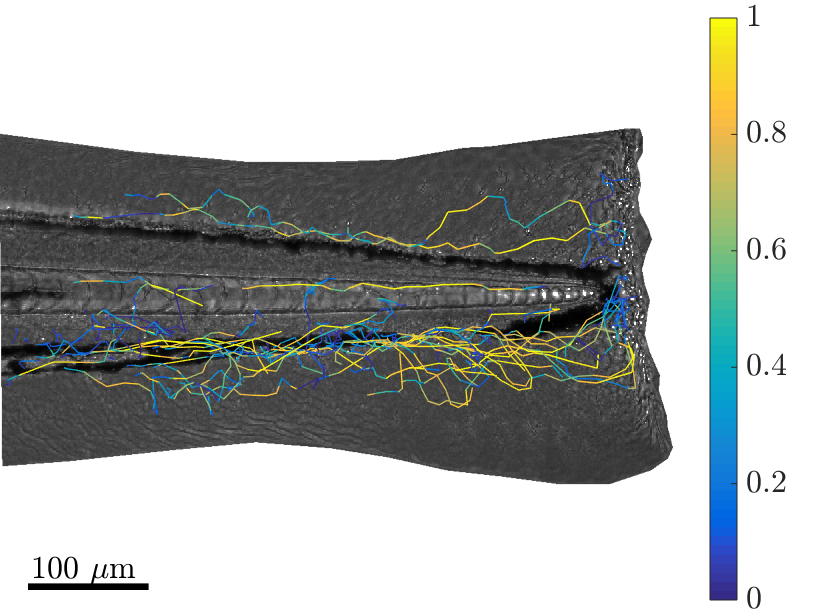
\includegraphics[scale=0.19]{Figures/mode1_fish3.png}
	\end{column}
	\begin{column}{0.31\textwidth}
		\vspace{-0.2cm}
		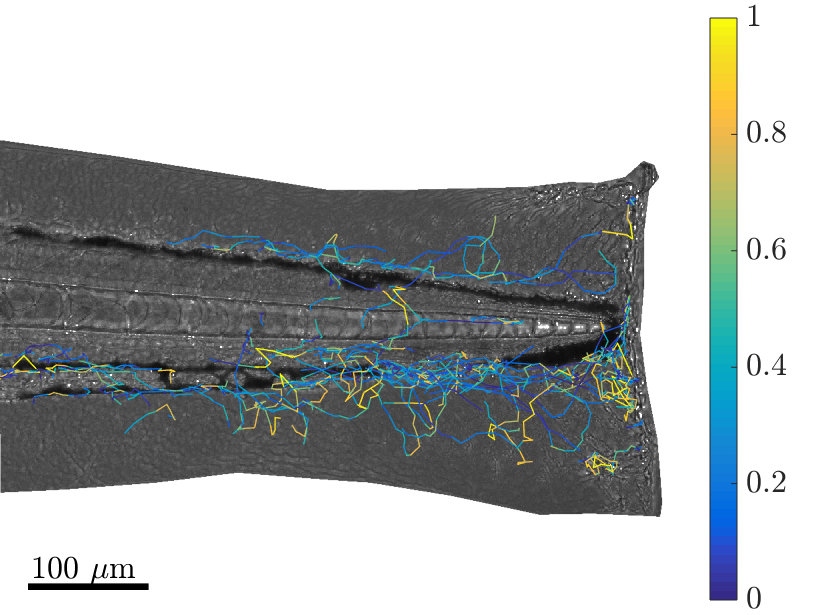
\includegraphics[scale=0.19]{Figures/mode2_fish1.png}\vfil
		\vspace{0.2cm}
		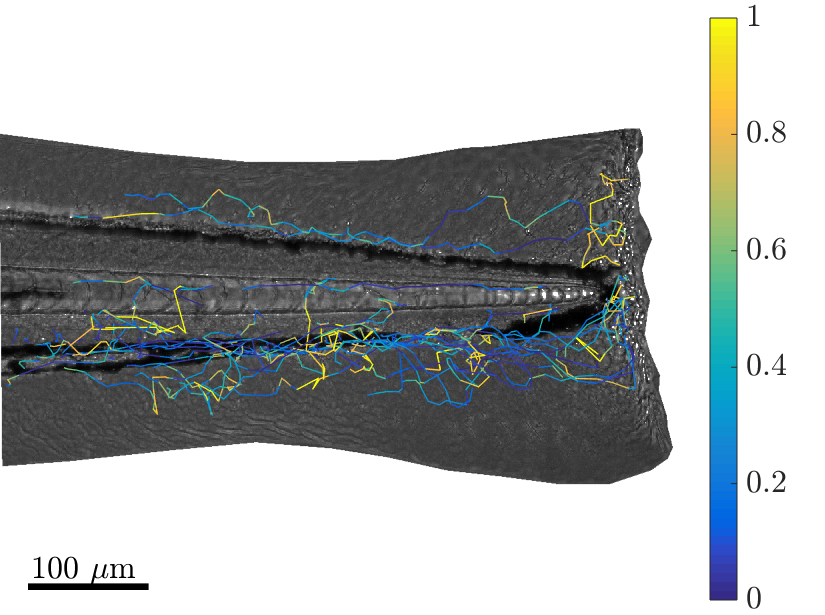
\includegraphics[scale=0.19]{Figures/mode2_fish3.png}
	\end{column}
	\begin{column}{0.31\textwidth}
		\vspace{-0.2cm}
		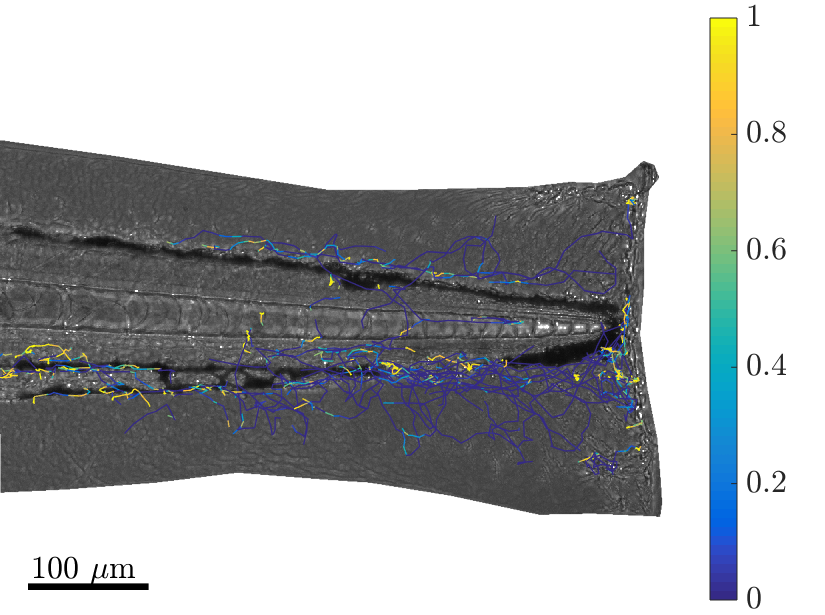
\includegraphics[scale=0.19]{Figures/mode3_fish1.png}\vfil
		\vspace{0.2cm}
		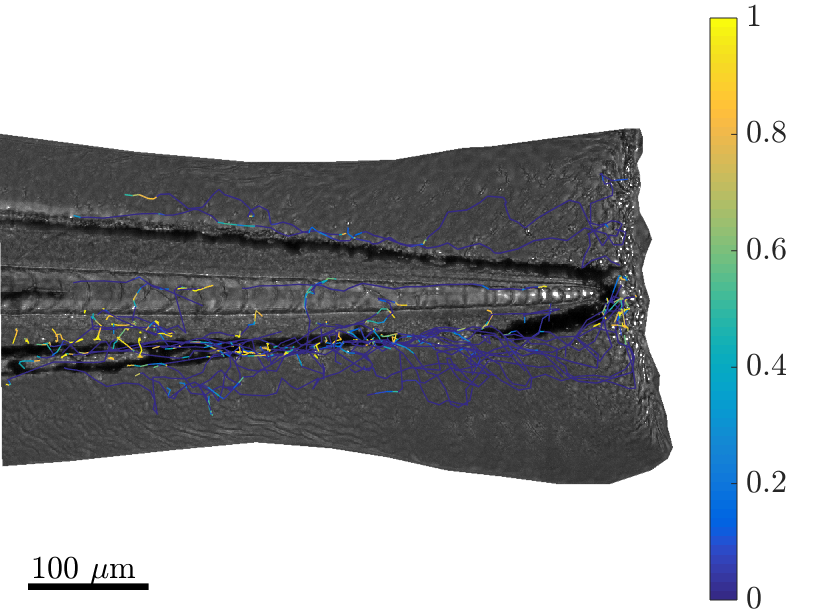
\includegraphics[scale=0.19]{Figures/mode3_fish3.png}
	\end{column}
\end{columns}
\begin{columns}
	\centering
	\begin{column}{0.31\textwidth}
		\centering
		\footnotesize{ a) $p(M^1)$}
	\end{column}
	\begin{column}{0.31\textwidth}
		\centering
		\footnotesize{ b)  $p(M^2)$}
	\end{column}
	\begin{column}{0.31\textwidth}
		\centering
		\footnotesize{ c)  $p(M^3)$}
	\end{column}
\end{columns}
\end{frame}
\begin{frame}{Migratory modes - severe and mild injury}
\begin{columns}
	\begin{column}{0.31\textwidth}
		\vspace{-0.2cm}
		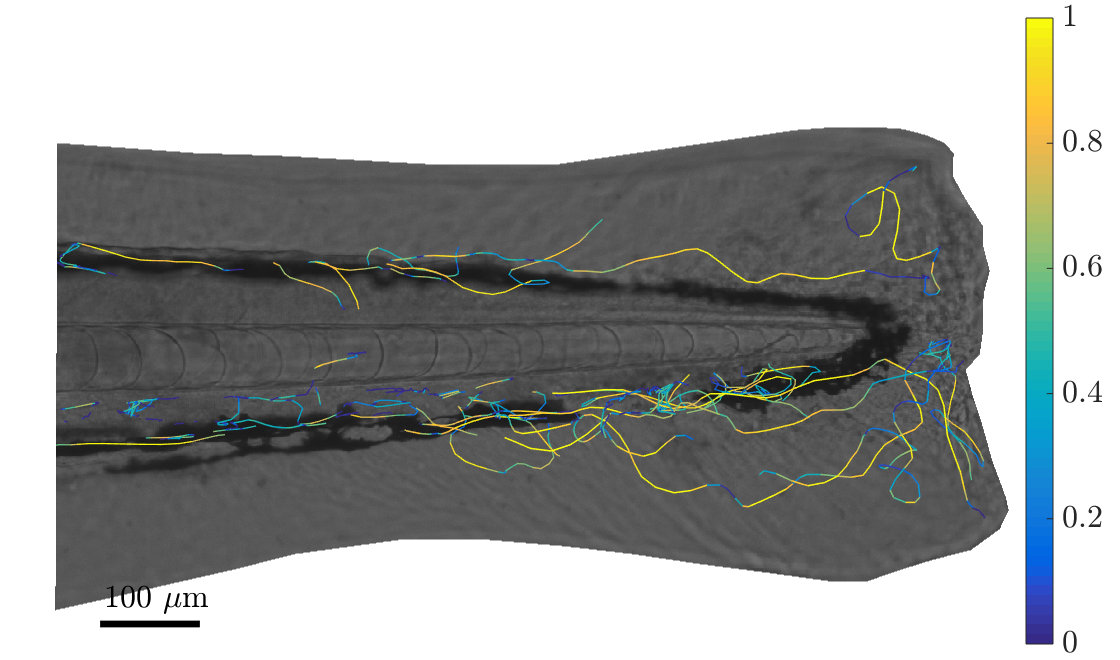
\includegraphics[scale=0.137]{Figures/mild1_mode1.png}\vfil
		\vspace{0.2cm}
		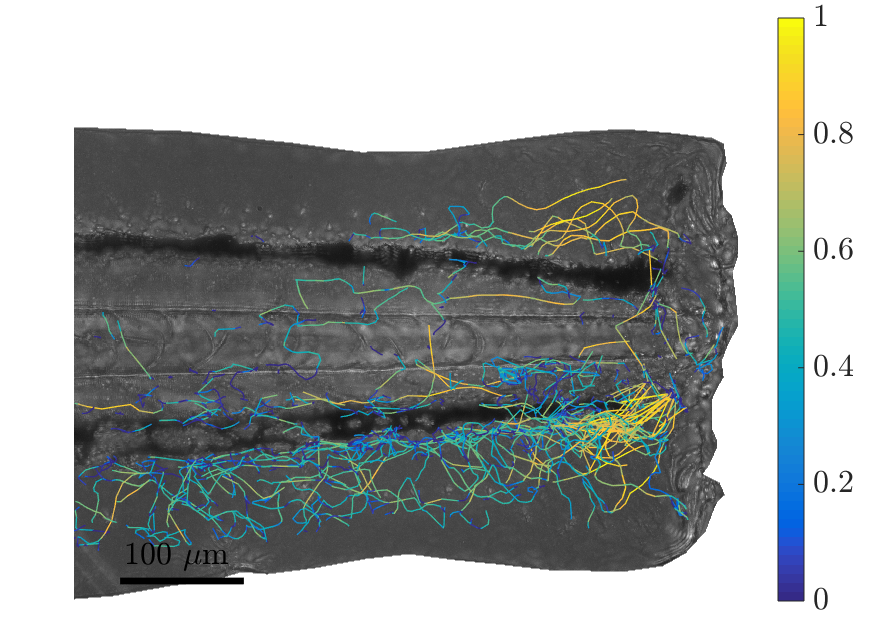
\includegraphics[scale=0.17]{Figures/severe1_mode1.png}
	\end{column}
	\begin{column}{0.31\textwidth}
		\vspace{-0.2cm}
		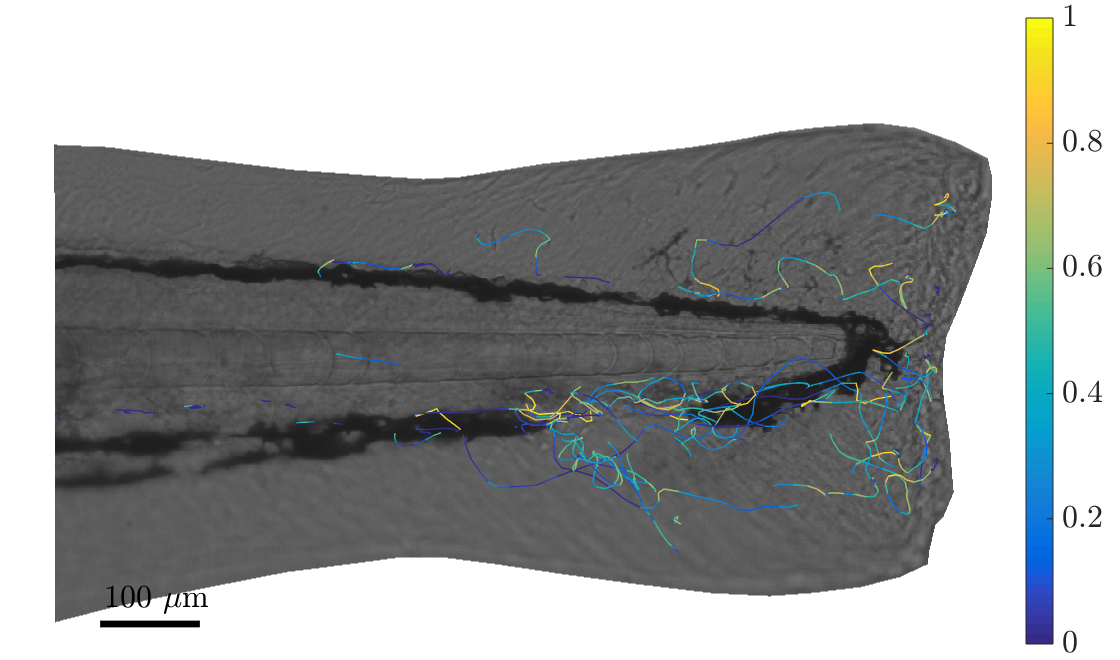
\includegraphics[scale=0.137]{Figures/mild1_mode2.png}\vfil
		\vspace{0.2cm}
		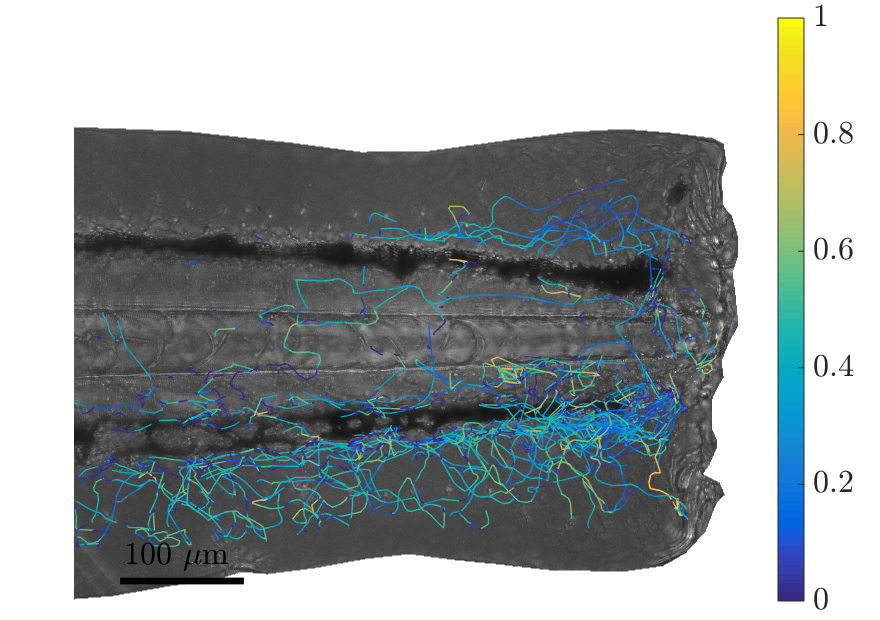
\includegraphics[scale=0.17]{Figures/severe1_mode2.png}
	\end{column}
	\begin{column}{0.31\textwidth}
		\vspace{-0.2cm}
		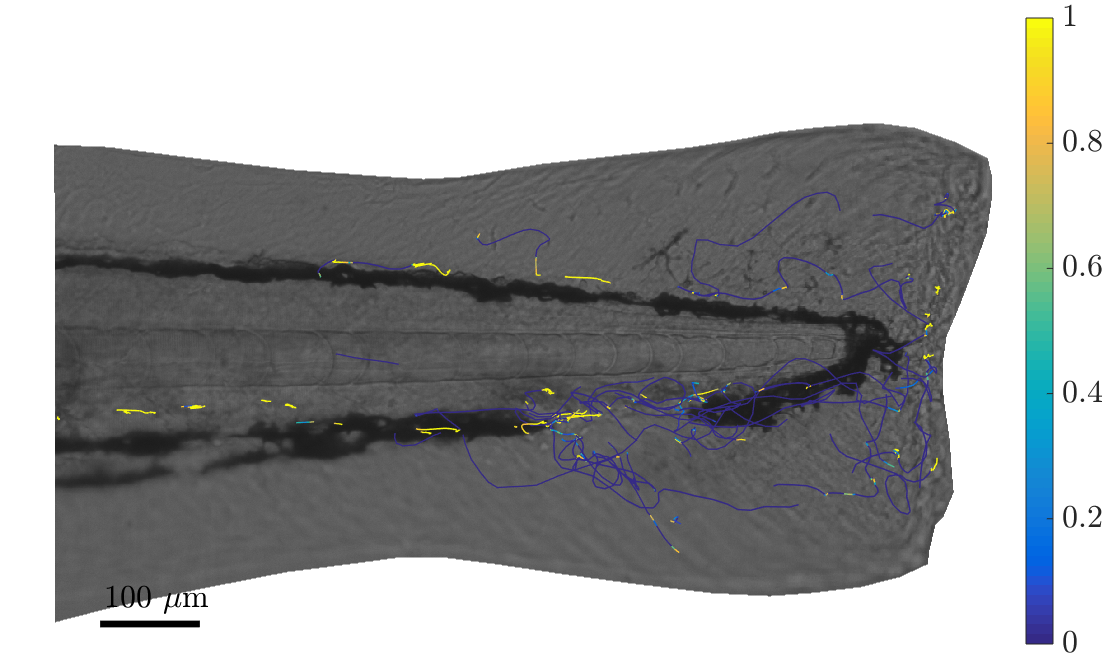
\includegraphics[scale=0.137]{Figures/mild1_mode3.png}\vfil
		\vspace{0.2cm}
		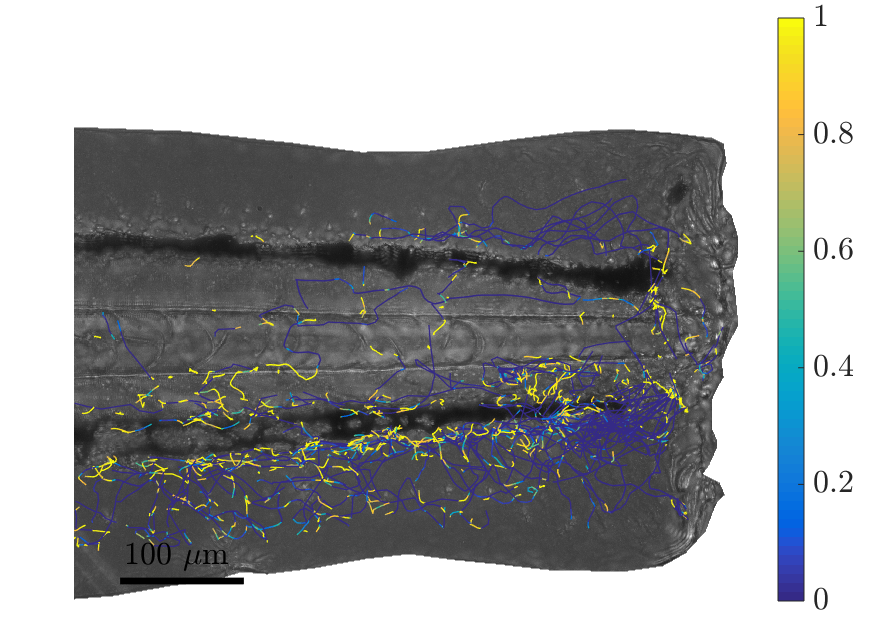
\includegraphics[scale=0.17]{Figures/severe1_mode3.png}
	\end{column}
\end{columns}
\begin{columns}
\centering
\begin{column}{0.31\textwidth}
	\centering
	\footnotesize{ a) $p(M^1)$}
\end{column}
\begin{column}{0.31\textwidth}
	\centering
	\footnotesize{ b)  $p(M^2)$}
\end{column}
\begin{column}{0.31\textwidth}
	\centering
	\footnotesize{ c)  $p(M^3)$}
\end{column}
\end{columns}
\end{frame}
\begin{frame}{Inferred chemoattractant environment}
\begin{columns}
	\begin{column}{0.3\textwidth}
		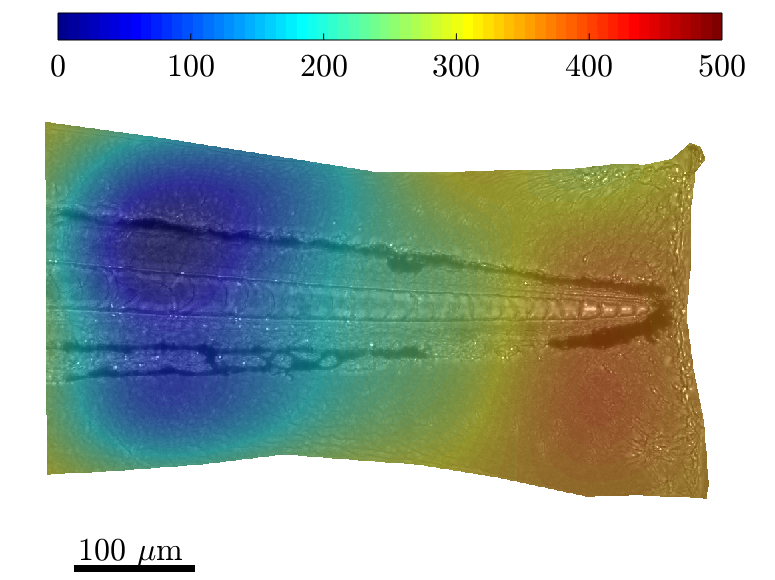
\includegraphics[scale=0.19]{Figures/field_fish1.png}
		\vspace{0.4cm}
		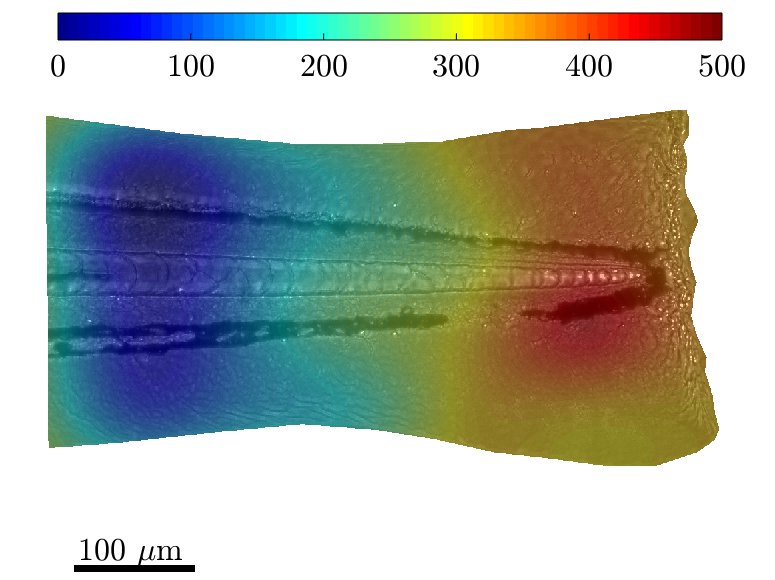
\includegraphics[scale=0.19]{Figures/field_fish3.png}
	\end{column}
	\begin{column}{0.3\textwidth}
		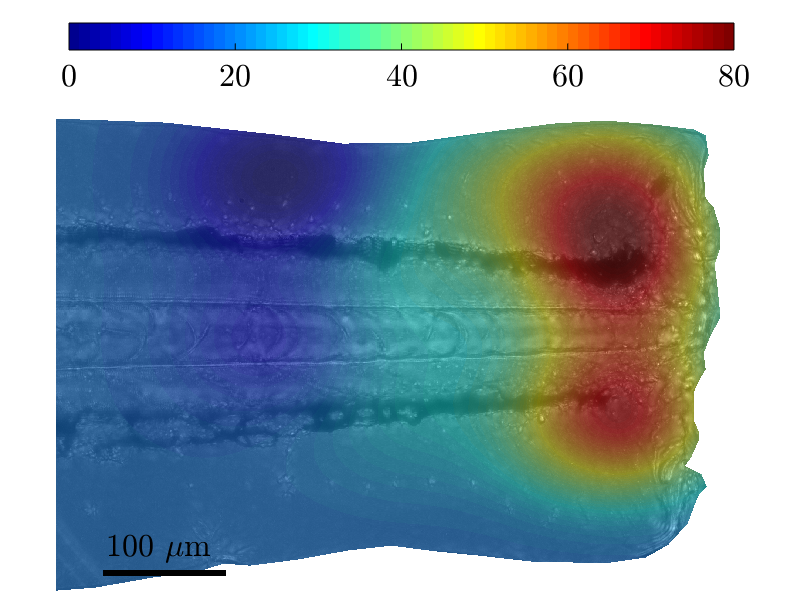
\includegraphics[scale=0.18]{Figures/severe1_field.png}
		\vspace{0.3cm}
		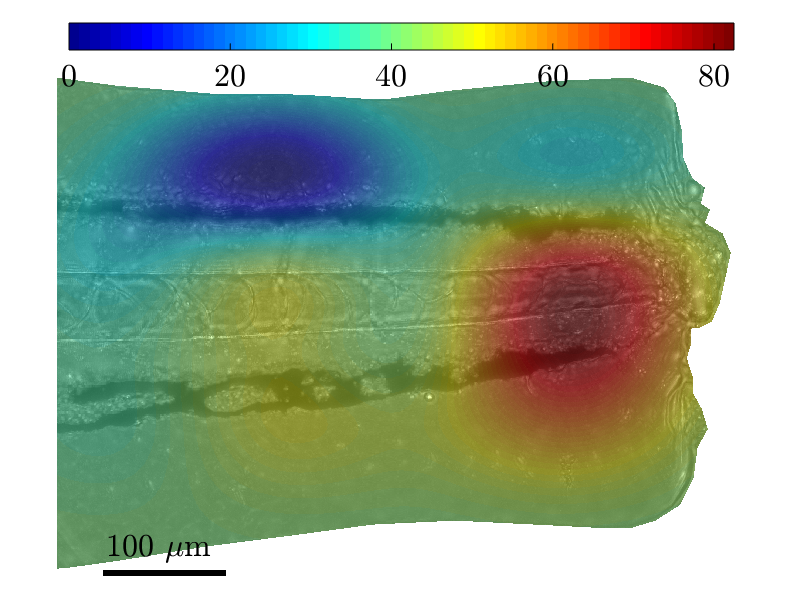
\includegraphics[scale=0.18]{Figures/severe2_field.png}
	\end{column}
	\begin{column}{0.3\textwidth}
		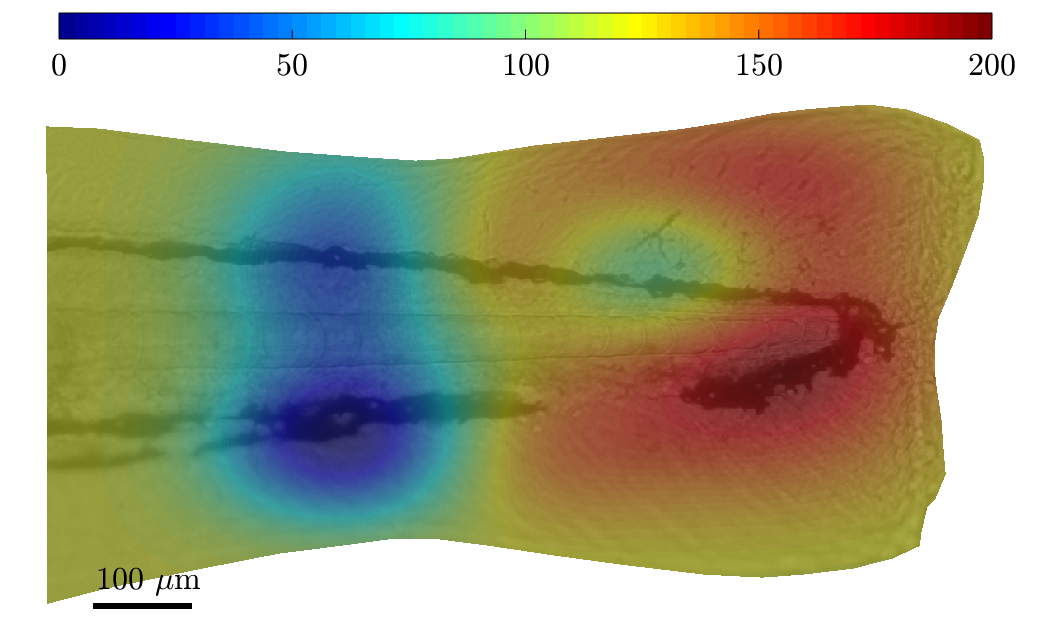
\includegraphics[scale=0.14]{Figures/mild1_field.png}
		\vspace{0.6cm}
		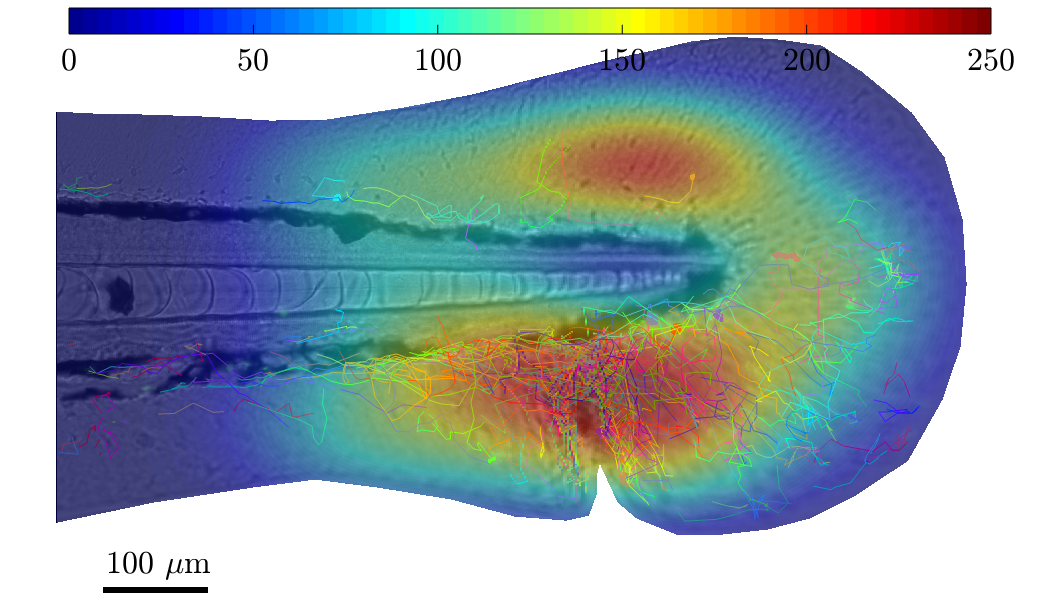
\includegraphics[scale=0.14]{Figures/nick4_field.png}
	\end{column}
\end{columns}
\begin{columns}
	\begin{column}{0.3\textwidth}
		\centering
		\footnotesize{ a) normal injury}
	\end{column}
	\begin{column}{0.3\textwidth}
		\centering
		\footnotesize{ b) severe injury}
	\end{column}
	\begin{column}{0.3\textwidth}
		\centering
		\footnotesize{ c) mild injury}
	\end{column}
\end{columns}
\end{frame}
\begin{frame}{Reverse migration}
\begin{columns}
	\begin{column}{0.31\textwidth}
		\vspace{-0.2cm}
		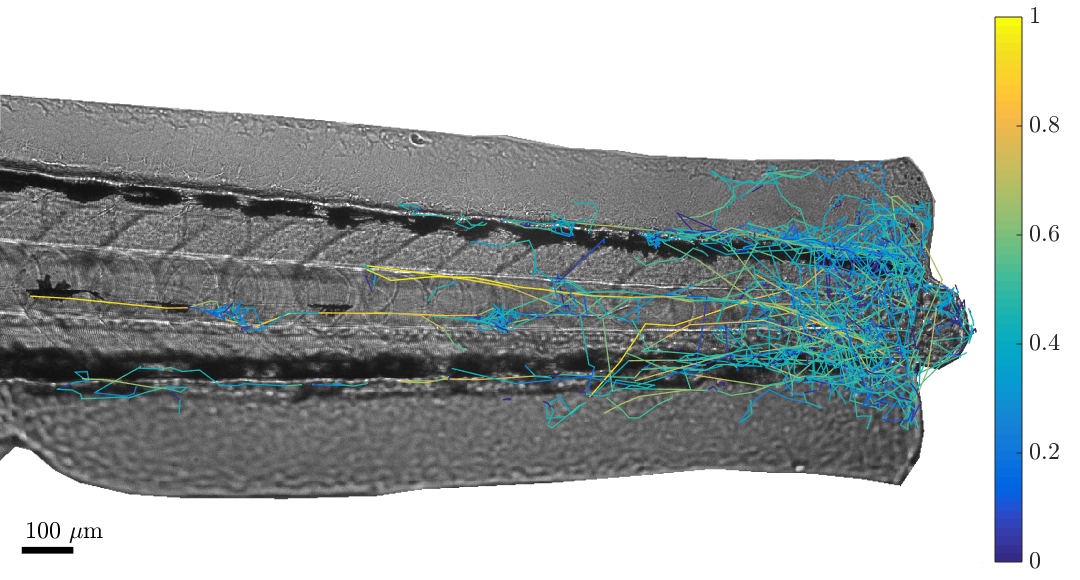
\includegraphics[scale=0.137]{Figures/mode1_rev2.png}\vfil
		\vspace{0.2cm}
		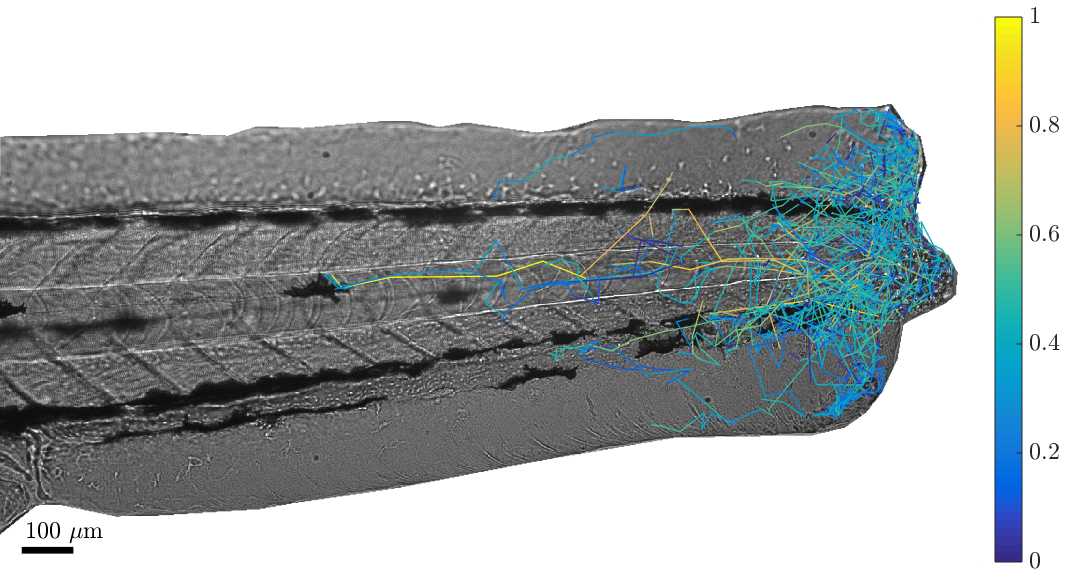
\includegraphics[scale=0.137]{Figures/mode1_rev9.png}
	\end{column}
	\begin{column}{0.31\textwidth}
		\vspace{-0.2cm}
		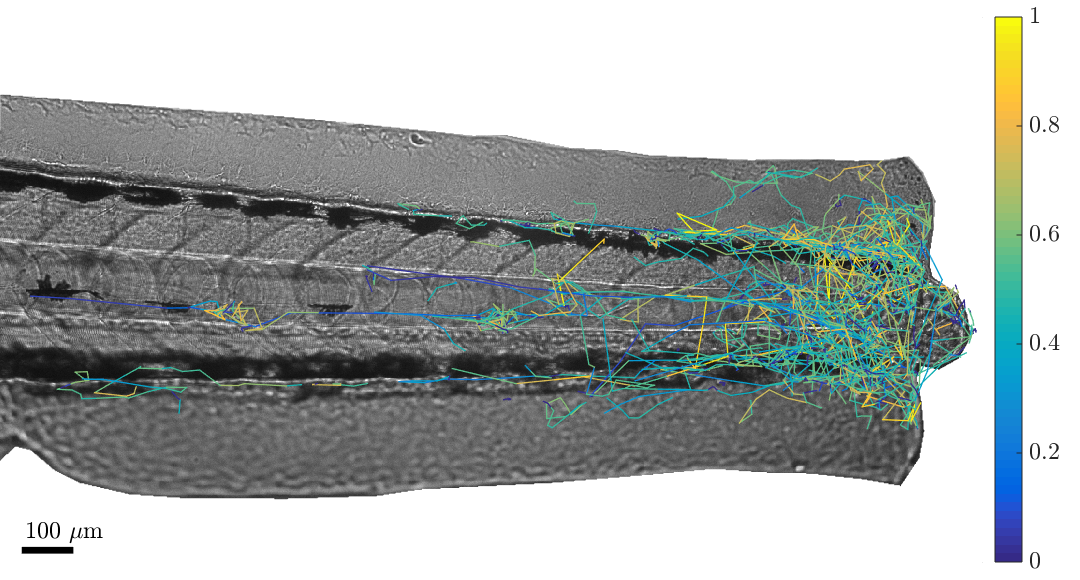
\includegraphics[scale=0.137]{Figures/mode2_rev2.png}\vfil
		\vspace{0.2cm}
		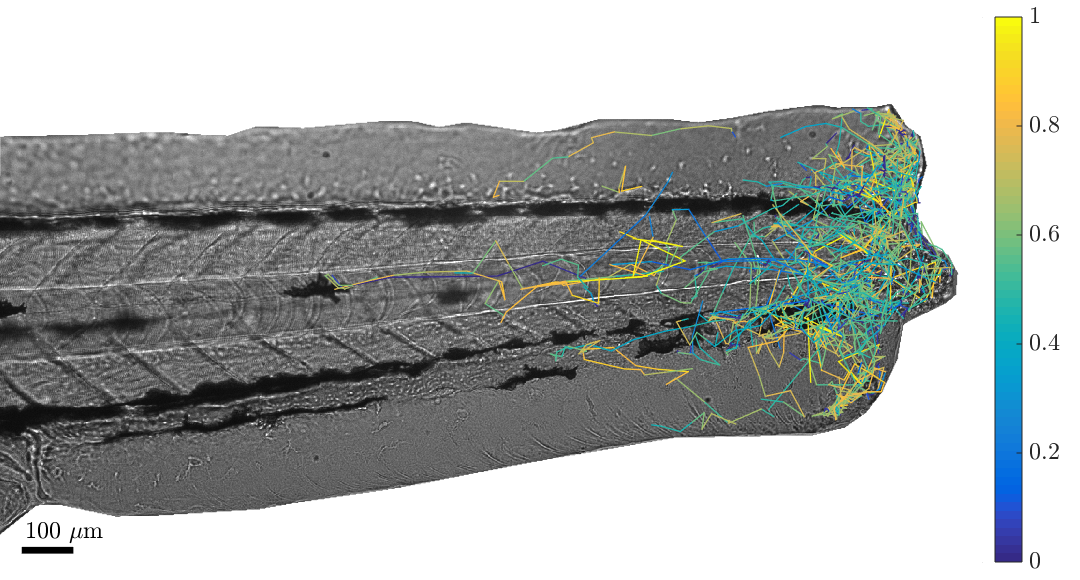
\includegraphics[scale=0.137]{Figures/mode2_rev9.png}
	\end{column}
	\begin{column}{0.31\textwidth}
		\vspace{-0.2cm}
		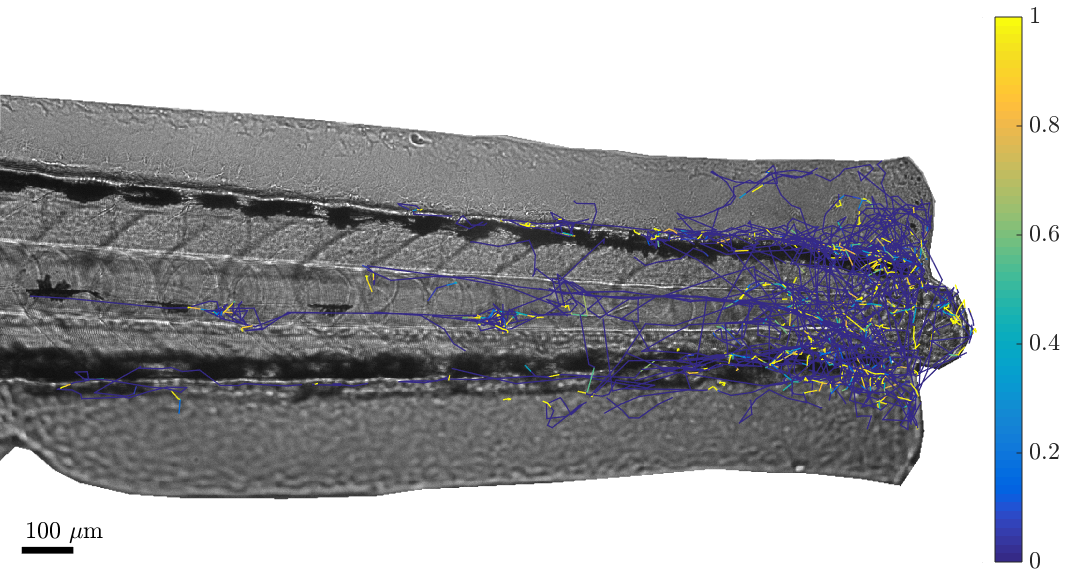
\includegraphics[scale=0.137]{Figures/mode3_rev2.png}\vfil
		\vspace{0.2cm}
		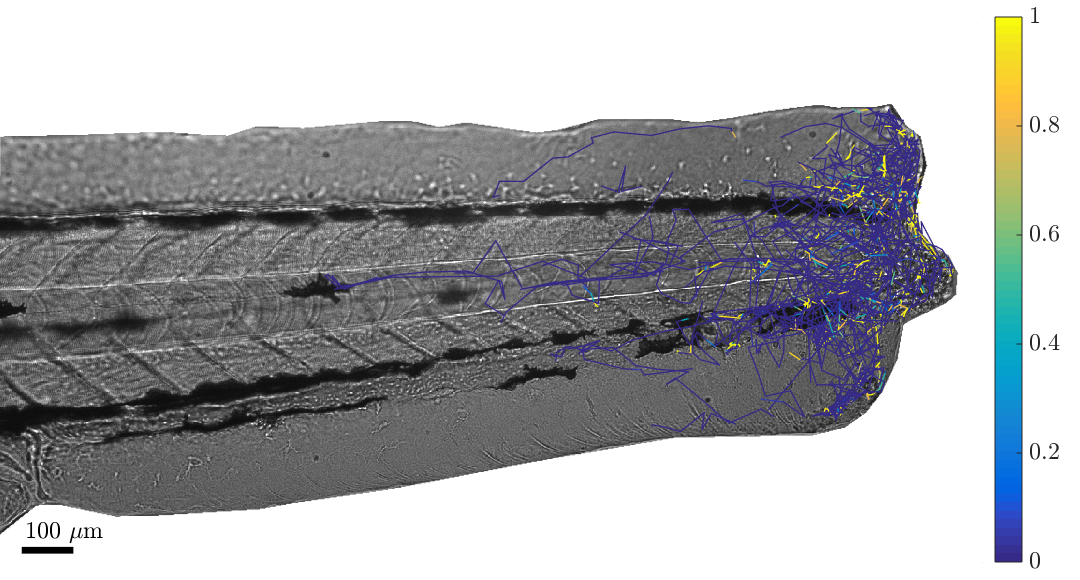
\includegraphics[scale=0.137]{Figures/mode3_rev9.png}
	\end{column}
\end{columns}
\vspace{0.5cm}
For 4 datasets there is higher probability of neutrophils diffusing away from the wound.
\end{frame}
\section{Estimating cell morphodynamics}
\subsection{Problem statement}
\begin{frame}
\begin{columns}
	\begin{column}{0.6\textwidth}
		\centering
		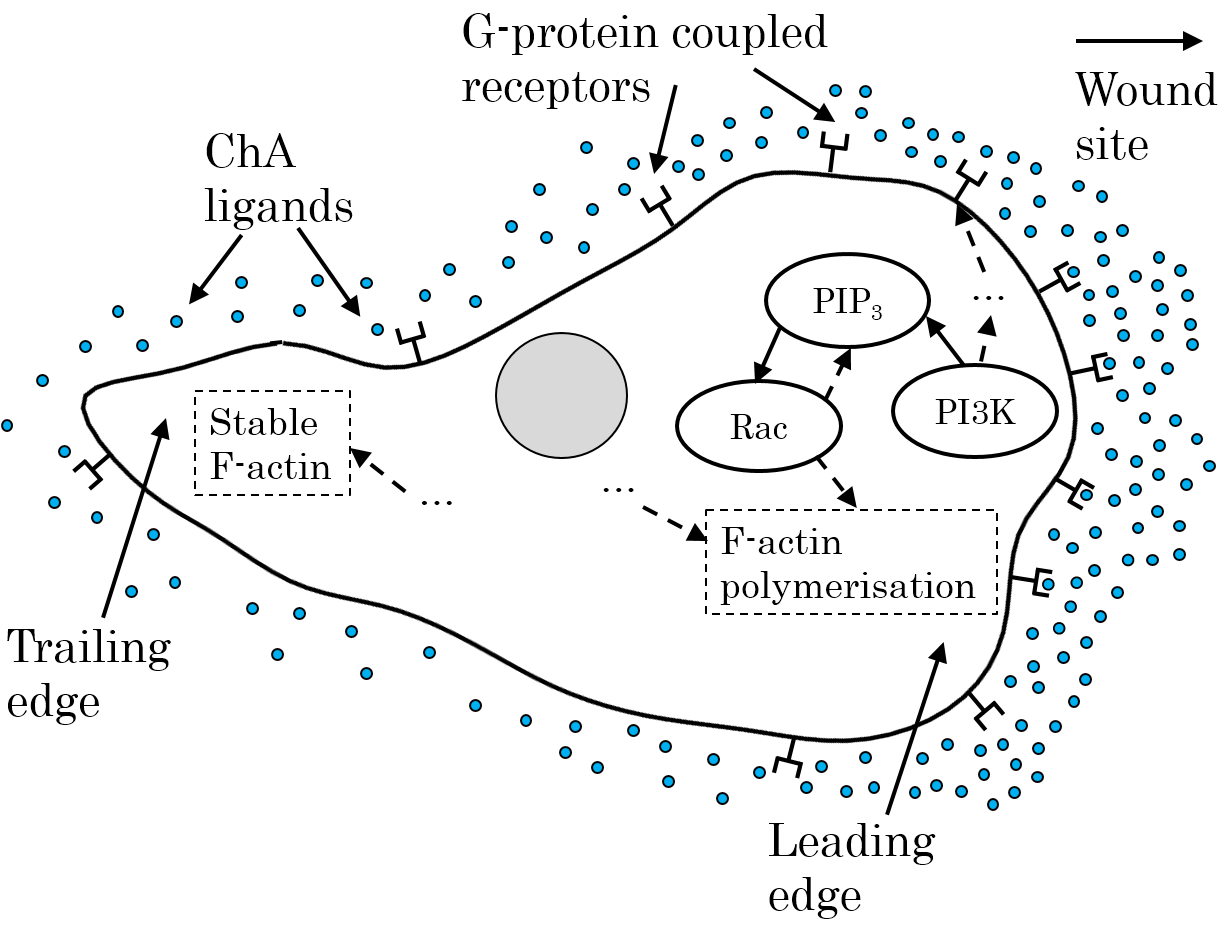
\includegraphics[scale=0.21]{Figures/sensing_neutrophil.png}
		\vfil		
	\end{column}
	\begin{column}{0.38\textwidth}
		\centering
		\scalebox{1}{	\input{Tikzes/RDS3.tikz}}
		\vfil
	\end{column}
\end{columns}
\bigskip
\uncover<2->{Does PIP$_3$ activate pseudopod growth?}
\end{frame}
\begin{frame}{Data}\centering
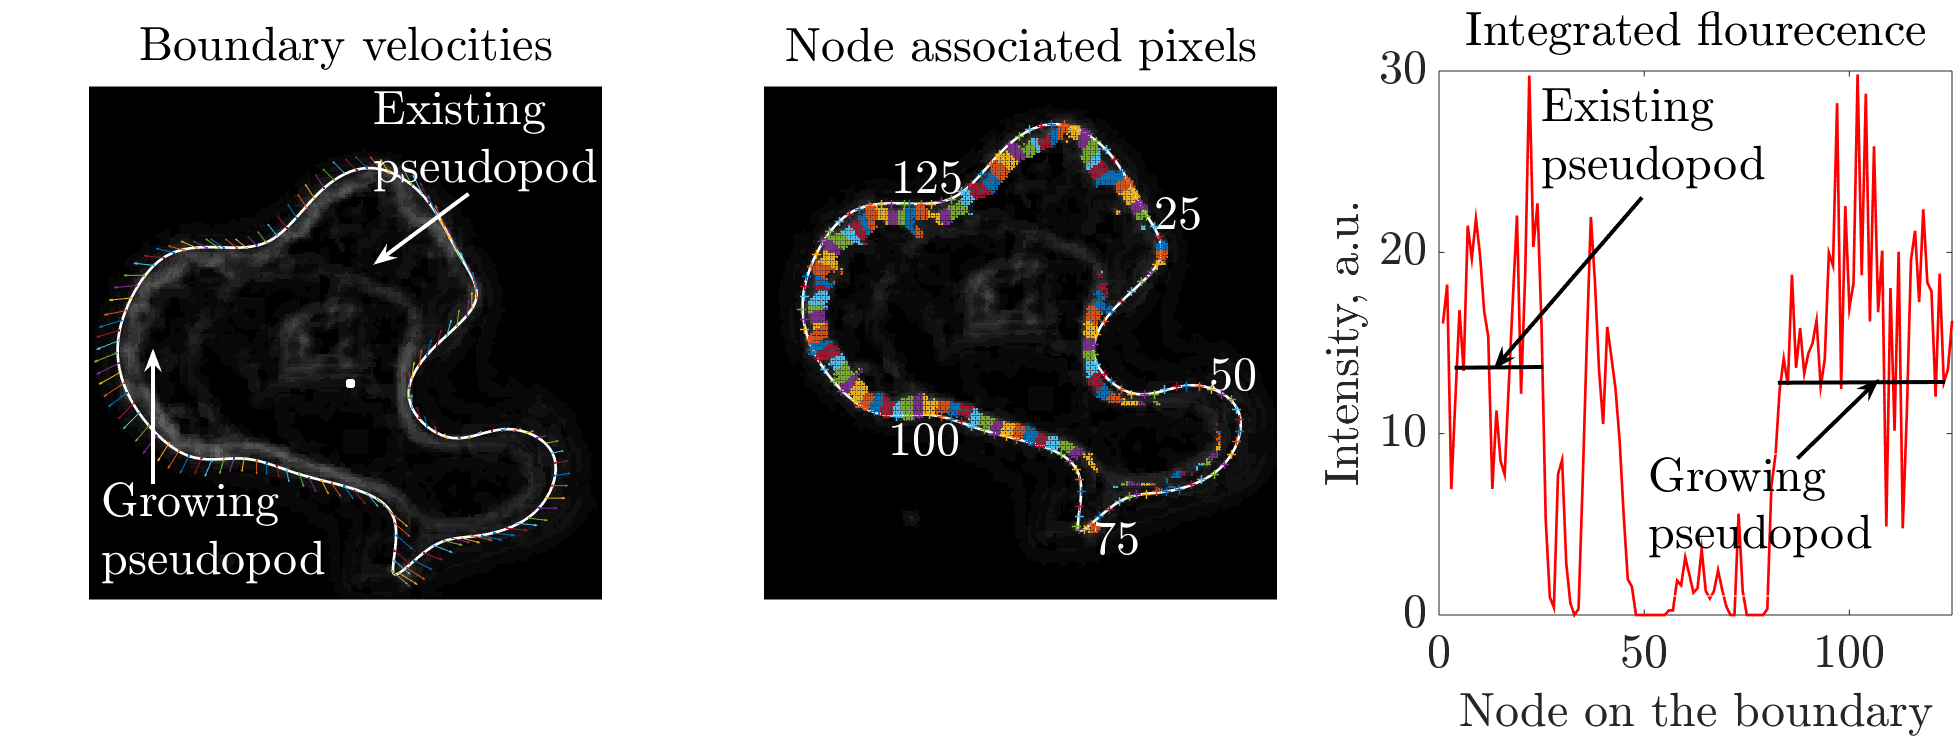
\includegraphics[scale=0.2]{Figures/motile_cell_t10.png}
\vfil
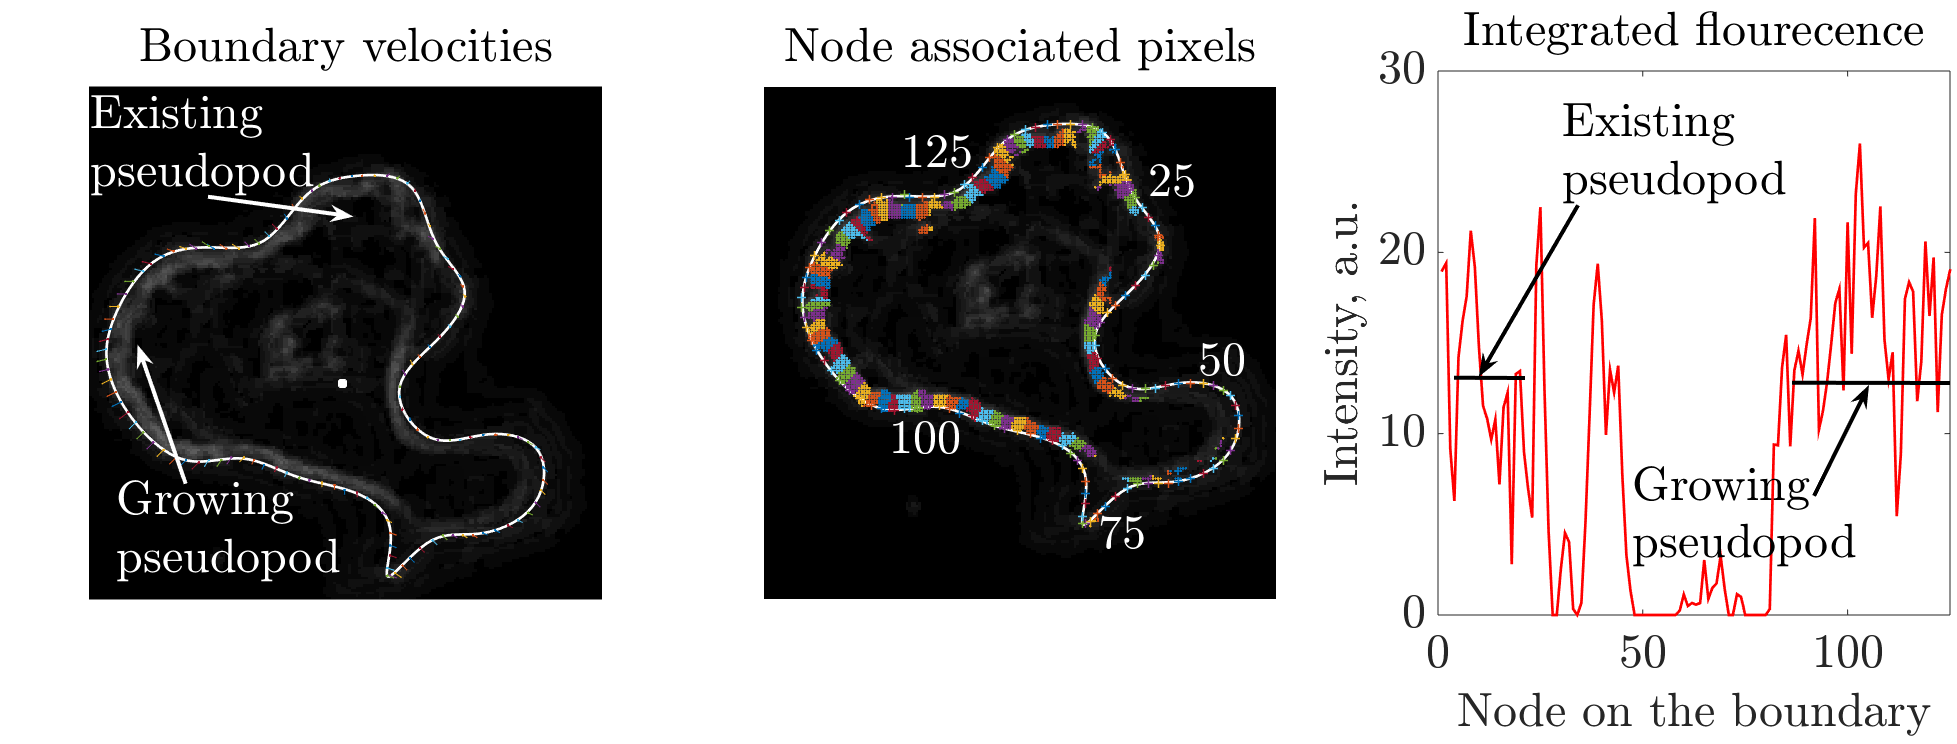
\includegraphics[scale=0.2]{Figures/motile_cell_t11.png}
\end{frame}
\begin{frame}{Defining assumptions}
\begin{itemize}
	\item PIP$_3$ is the only activator regulating the cell membrane protrusion.
	\item The integrated 
fluorescence intensity obtained from the imaging data is proportional to the local PIP$_3$ concentration.
	\item Local shape change is fully described by normal velocity.
	\item The cell is flat.
\end{itemize}
\end{frame}
\subsection{Methods}
\begin{frame}{Forces acting on cell boundary}
\vspace{-0.5cm}
\begin{equation*}
\mathcal{F} = (\mathcal{F}_{\textrm{visc}} + \mathcal{F}_{\textrm{pro}} + \mathcal{F}_{\textrm{ten}} + \mathcal{F}_{\textrm{vol}})\nu,
\end{equation*}
\begin{itemize}
	\item \textbf{\textit{Protrusive force}} proportional to concentration of species active along the cell boundary: \begin{equation*}
	\mathcal{F}_{\textrm{pro}} = \alpha_{\textrm{pro}}a_{\td}^{k}.
	\end{equation*}
	\item \textbf{\textit{Surface tension}} corresponds to surface energy that prevents cell membrane from stretching:
	\begin{equation*}
	\mathcal{F}_{\textrm{ten}} = \alpha_{\textrm{ten}} \kappa_{\td}^{k}.
	\end{equation*} 
	\item \textbf{\textit{Volume conservation}} balances small volume changes:
	\begin{equation*}
	\mathcal{F}_{\textrm{vol}} = \alpha_{\textrm{vol}}\Delta\mathcal{A}_{\td}.
	\end{equation*} 
	\item \textbf{\textit{Viscous force}} opposes cell motion:
	\begin{equation*}
	\mathcal{F}_{\textrm{visc}} = -\alpha_{\textrm{vv}}\mathbfit{v}_{\td}^{k}.
	\end{equation*}
\end{itemize}
$\quad$\\
$\quad$
\end{frame}
\begin{frame}{State space model}
Cell boundary is represented by a discrete polygon with $K$ vertexes. Local evolution for each vertex:
\begin{equation*}
\mathbfit{v}_{\td+1}^{k} = A\mathbfit{v}_{\td}^{k} + B\mathbfit{u}_{\td}^{k}+ \mathbfit{w}_{\td}^{k}, \quad \mathbfit{w}{\td}^{k} \sim \mathcal{N}(0,Q).
\end{equation*}
\begin{equation*}
\mathbfit{y}_{\td}^{k} = C \mathbfit{v}_{\td}^{k}.
\end{equation*}
\begin{itemize}
\item 
$A = 1 - \alpha_{\textrm{vv}}$;
$B = \left[\alpha_{\textrm{pro}}, \alpha_{\textrm{ten}}, \alpha_{\textrm{vol}}\right]$;
\item 
$\mathbfit{u}_{\td}^{k} =\left[  a_{\td}^{k}, \kappa_{\td}^{k}, \Delta\mathcal{A}_{\td} \right] ^\top$, where
	\begin{itemize}
		\item $a_{\td}^{k}$ - local concentration of PIP$_3$;
		\item $\kappa_{\td}^{k}$ - local curvature;
		\item $\Delta\mathcal{A}_{\td} = \mathcal{A}_{\td} - \mathcal{A}_0$ - change in cell shape. 
	\end{itemize}
\item $\Theta = \lbrace A, B, Q, \mathbfit{v}_0, P_0 \rbrace$ - estimated via classic EM algorithm.
\end{itemize}
\end{frame}


%\begin{frame}
%\begin{columns}
%	\begin{column}{0.5\textwidth}
%		\begin{figure}
%			\scalebox{0.8}{\input{Tikzes/vertnormals.tikz}}
%			\caption{\small Cell normals.} 
%		\end{figure}
%	\end{column}
%	\begin{column}{0.5\textwidth}
%		\begin{figure}
%			\scalebox{0.8}{\input{Tikzes/area1.tikz}}
%			\caption{Cell area computation.} 
%		\end{figure}
%	\end{column}
%\end{columns}
%\end{frame}



%\begin{frame}
%\begin{columns}
%	\begin{column}{0.5\textwidth}
%		\begin{figure}
%			\scalebox{0.6}{\input{Tikzes/normvelt3.tikz}}
%			\vfil
%			\scalebox{0.6}{\input{Tikzes/normvelt4.tikz}}
%			\caption{\small Normal velocities.} 
%		\end{figure}
%	\end{column}
%	\begin{column}{0.5\textwidth}
%		\begin{figure}
%			\scalebox{0.465}{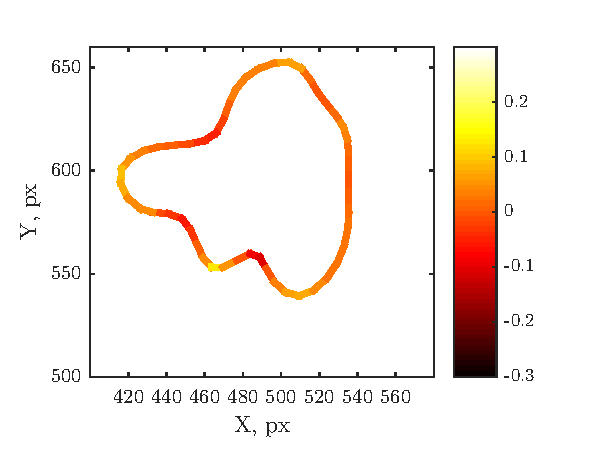
\includegraphics{Figures/curv3.eps}}
%			\vfil
%			\scalebox{0.465}{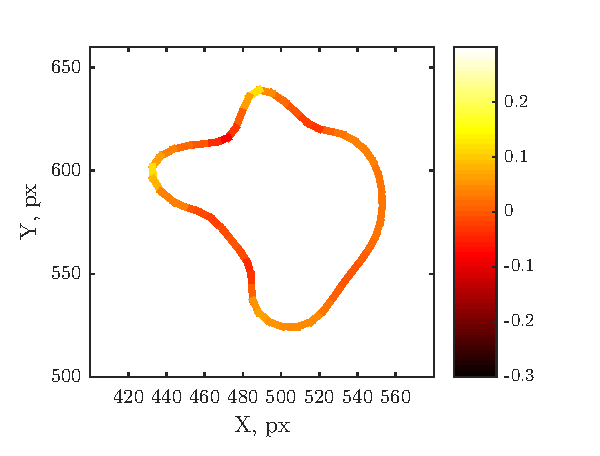
\includegraphics{Figures/curv4.eps}}
%			\caption{\footnotesize Local curvature.} 
%		\end{figure}
%	\end{column}
%\end{columns}
%\end{frame}

\subsection{Selected results}
\begin{frame}{Motile cells observed in vivo}
\begin{columns}
	\begin{column}{0.48\textwidth}
		\centering
		\scalebox{0.6}{\input{Tikzes/histogram7.tikz}}	
	\end{column}
	\begin{column}{0.52\textwidth}
		\centering
		\begin{itemize}
			\item Very weak correlation between between $a_{\td-1}^{k}$ and $\mathbfit{v}_{\td}^{k}$;
			\item Correlation coefficients are inconsistent for different cells in the same set;
			\item Mann-Whitney test results: on average, higher concentration of PIP$_3$ accelerates protrusion growth, but does not activate it.
		\end{itemize}
	\end{column}
\end{columns}
\end{frame}
\begin{frame}{Motile cells observed in vivo}
\begin{columns}
	\begin{column}{0.5\textwidth}
		\centering
		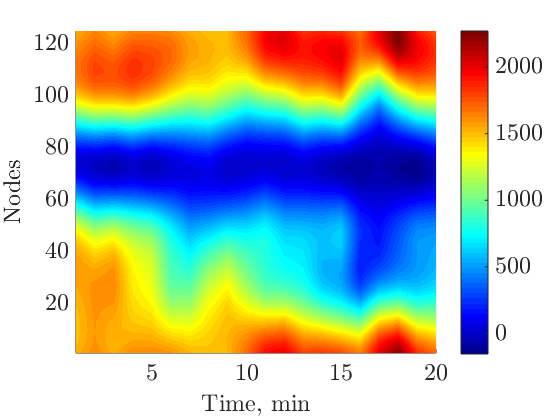
\includegraphics[scale=0.3]{Figures/m4_akt.png}\vfil
		\footnotesize{a) Smoothed intensity.}
		\vfil
		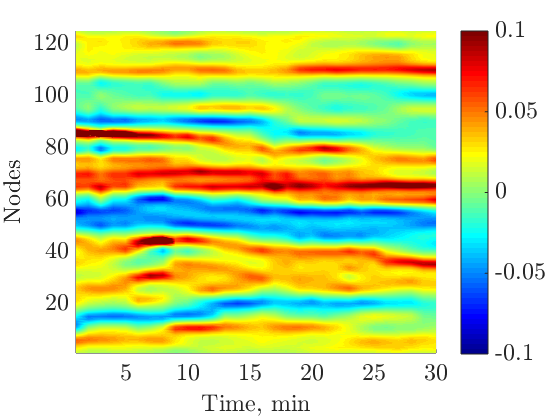
\includegraphics[scale=0.3]{Figures/m4_curvature.png}\vfil	
		\footnotesize{a) Local curvature.}
	\end{column}
	\begin{column}{0.5\textwidth}
		\centering
		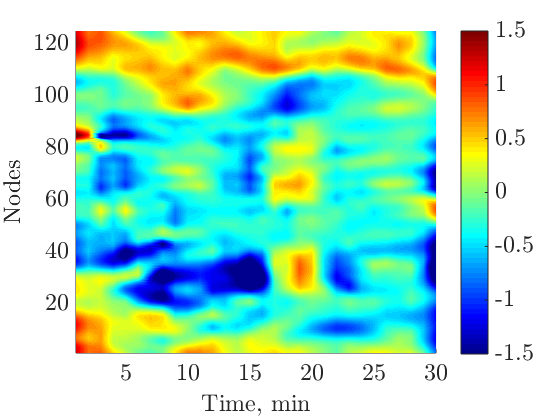
\includegraphics[scale=0.3]{Figures/m4_estimated_velocity.png}\vfil
		\footnotesize{c) Estimated velocity.}
		\vfil
		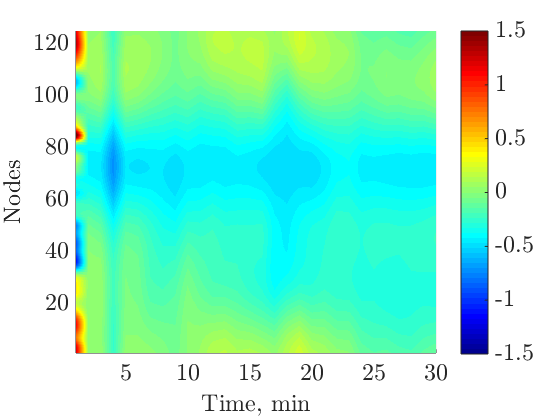
\includegraphics[scale=0.3]{Figures/m4_modelled_velocity.png}\vfil
		\footnotesize{d) Predicted velocity.}
	\end{column}
\end{columns}
\end{frame}
\begin{frame}{Polarised cell observed in vitro}
\centering
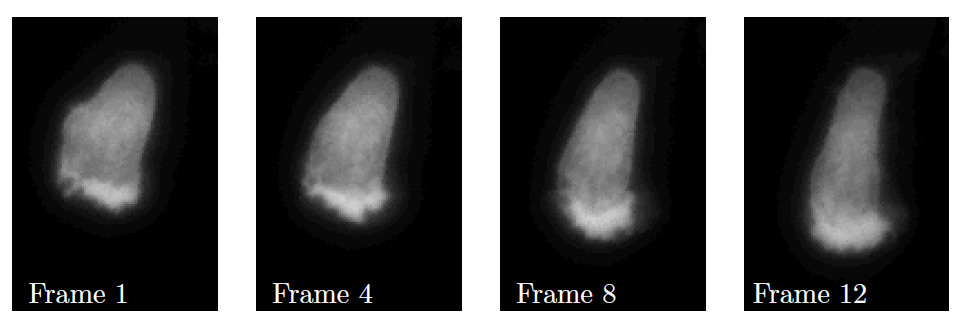
\includegraphics[scale=0.4]{Figures/in_vitro_cell.png}
\vfil
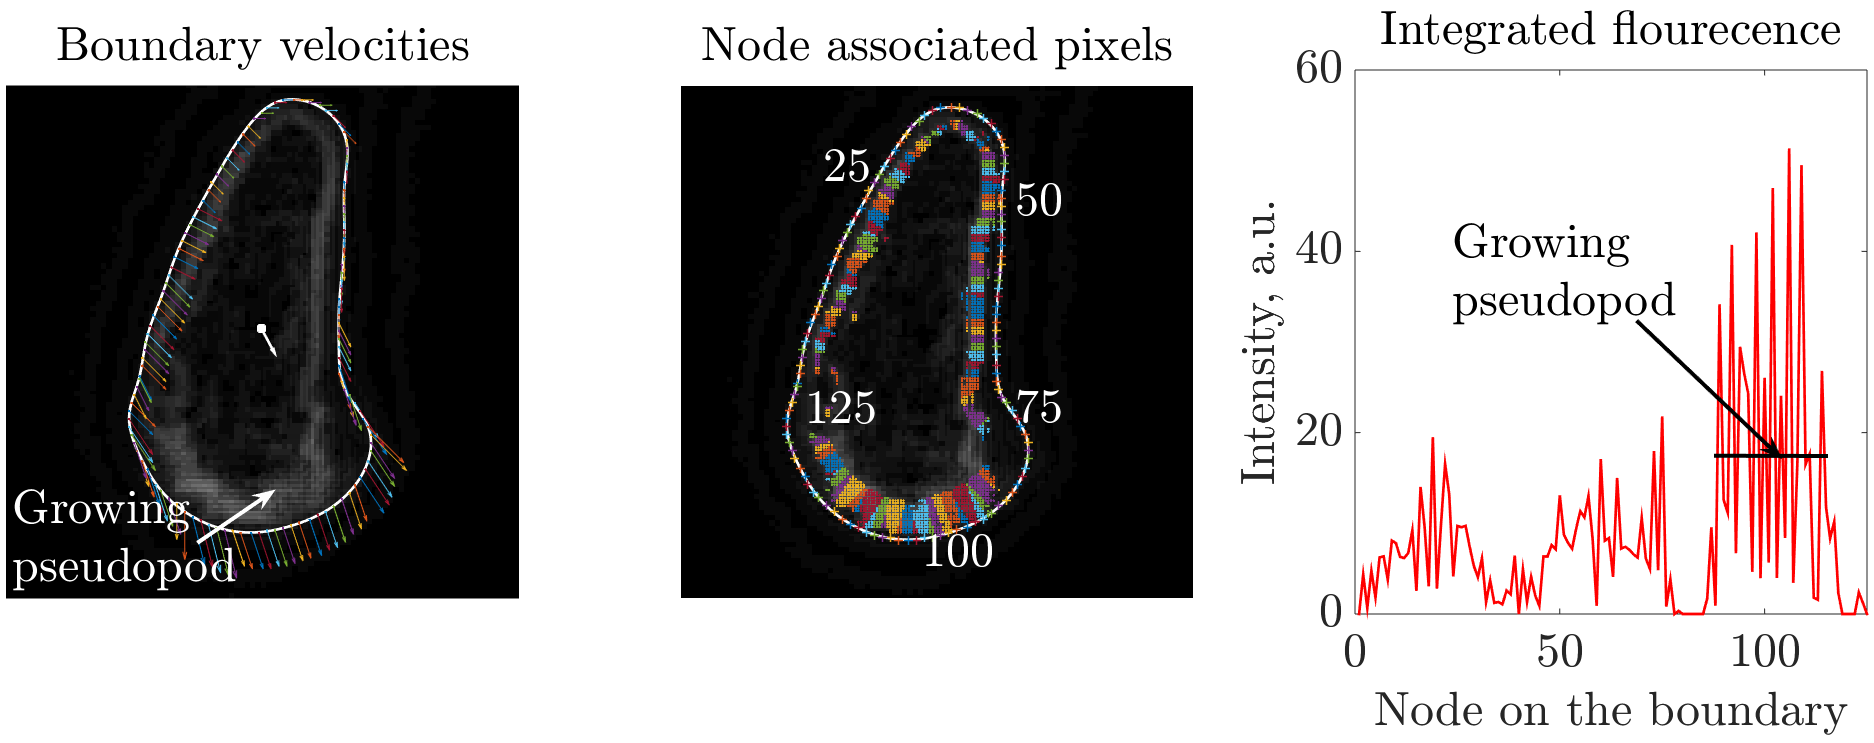
\includegraphics[scale=0.2]{Figures/normally_polarised_t9.png}
\end{frame}
\begin{frame}{Polarised cell observed in vitro}
\begin{columns}
	\begin{column}{0.5\textwidth}
	\centering
	\includegraphics[scale=0.3]{Figures/polarised_smoothed_akt.png}\vfil
	\footnotesize{a) Smoothed intensity.}
	\vfil
	\includegraphics[scale=0.3]{Figures/polarised_curvature.png}\vfil	
	\footnotesize{a) Local curvature.}
\end{column}
\begin{column}{0.5\textwidth}
	\centering
	\includegraphics[scale=0.3]{Figures/polarised_estimated_velocity.png}\vfil
	\footnotesize{c) Estimated velocity.}
	\vfil
	\includegraphics[scale=0.3]{Figures/polarised_modelled_velocity.png}\vfil
	\footnotesize{d) Predicted velocity.}
\end{column}
\end{columns}
\end{frame}



\section{Conclusion}
\subsection{Contributions}
\begin{frame}{Technical contributions}
\begin{itemize}
	\item A reconfigurable hybrid model of individual cell dynamics that incorporates the influence of the global chemoattractant environment.
	\item A statistical framework for simultaneous inference of the global chemoattractant environment and cell behavioural modes from cell tracking data.
	\item An image processing and estimation framework that links local cell boundary evolution to observed subcellular concentrations.
\end{itemize}
\end{frame}
\begin{frame}{Contributions in field of application}
\begin{itemize}
	\item Investigation of cell-environment interaction on different stages of inflammation.
	\item Quantitative evidence that the dominant mode of neutrophil reverse migration is random walk.
	\item Quantitative evidence that PIP$_3$ does not activate protrusions but accelerates existing leading edges in cells performing chemotaxis.
\end{itemize}
\end{frame}
\subsection{Future work}
\begin{frame}{Future work}
\begin{itemize}
	\item Utilising hierarchical/multi-resolution basis functions in environment decomposition.
	\item Introducing priors for the field parameters and Bayesian inference.
	\item Considering time-varying environment for recruitment stage of inflammation.
	\item Considering competing gradients for resolution stage of inflammation.
	\item Shorten this presentation.
\end{itemize}
\end{frame}
\begin{frame}{Disseminated results}
\footnotesize{
\begin{itemize}
\item A. Kadochnikova, H.M. Isles, S.A. Renshaw, V. Kadirkamanathan.
"Estimation of Hidden Chemoattractant Field from Observed Cell Migration Patterns". A peer-reviewed paper in \textit{Proceedings of 18th IFAC Symposium on System Identification SYSID 2018}.
\item H.M. Isles, C. Muir, A. Kadochnikova, C.A. Loynes, V. Kadirkamanathan, P.M. Elks, S.A. Renshaw. "Non-apoptotic pioneer neutrophils initiate a swarming response in a zebrafish tissue injury model" under review in eLife Reports, 2019.
\end{itemize} 
In preparation:
\begin{itemize}
	\item A. Kadochnikova, V. Kadirkamanathan.
	"An Approximate Maximum Likelihood Framework for Estimating the Environment Driving multiple objects with Hybrid Dynamics".
	\item A. Kadochnikova, H.M. Isles, S.A. Renshaw, V. Kadirkamanathan. "Inference of the
	External Stimuli Environments from Heterogeneous Behaviour of Migrating Neutrophils in Zebrafish Model of Inflammation".
\end{itemize}
}
\end{frame}
\begin{frame}
\centering
\Huge{Thank you!}\\
\huge{Questions?}
\end{frame}
% All of the following is optional and typically not needed. 
%\appendix
%\section<presentation>*{\appendixname}
%\subsection<presentation>*{References}
%
%\begin{frame}[allowframebreaks]
%\printbibliography
%\end{frame}
\end{document}


